%%%%%%%%%%%%%%%%%%%%%%%%%%%%%%%%%%%%%%%%%%%%%%%%%%%
%% LaTeX book template                           %%
%% Author:  Amber Jain (http://amberj.devio.us/) %%
%% License: ISC license                          %%
%%%%%%%%%%%%%%%%%%%%%%%%%%%%%%%%%%%%%%%%%%%%%%%%%%%

\documentclass{report}
%\usepackage[letterpaper,margin=1in]{geometry} %showframe,pass
\usepackage[T1]{fontenc}
\usepackage[utf8]{inputenc}
\usepackage{lmodern}
\usepackage{longtable}
\usepackage{multirow}
\usepackage{hyperref}
\usepackage{changepage}
\usepackage{listings}
%\usepackage{authblk}
\usepackage{indentfirst}
\usepackage{marginnote}
\usepackage{enumitem}
\usepackage{setspace}
\usepackage{forest}
\usepackage{booktabs}
\usepackage{adjustbox}
% \usepackage{biblatex}
\usepackage{tcolorbox}
\usepackage{bm}
\usepackage{xspace}
\usepackage{etoolbox }
\usepackage{subcaption}


\usepackage{kpfonts}
\usepackage[T1]{fontenc}

\tcbuselibrary{listings,skins}

\usepackage{color}
\usepackage[a4paper, margin=1.2in]{geometry}
%%%%%%%%%%%%%%%%%%%%%%%%%%%%%%%%%%%%%%%%%%%%%%%%%%%%%%%%%
% Source: http://en.wikibooks.org/wiki/LaTeX/Hyperlinks %
%%%%%%%%%%%%%%%%%%%%%%%%%%%%%%%%%%%%%%%%%%%%%%%%%%%%%%%%%
\usepackage{hyperref}
\usepackage{graphicx}
\usepackage[english]{babel}



\usepackage{bera}% optional: just to have a nice mono-spaced font
\usepackage{xcolor}

\newcommand\JSONnumbervaluestyle{\color{blue}}
\newcommand\JSONstringvaluestyle{\color{red}}

% switch used as state variable
\newif\ifcolonfoundonthisline

\makeatletter


\newrobustcmd{\muferro}{$\bm{\mu}$-Ferro\xspace}
\newrobustcmd{\mupro}{$\bm{\mu}$-Pro\textsuperscript{\textregistered}\xspace}

\definecolor{folderbg}{RGB}{124,166,198}
\definecolor{folderborder}{RGB}{110,144,169}

\def\Size{4pt}
\tikzset{
      folder/.pic={
        \filldraw[draw=folderborder,top color=folderbg!50,bottom color=folderbg]
          (-1.05*\Size,0.2\Size+5pt) rectangle ++(.75*\Size,-0.2\Size-5pt);  
        \filldraw[draw=folderborder,top color=folderbg!50,bottom color=folderbg]
          (-1.15*\Size,-\Size) rectangle (1.15*\Size,\Size);
      }
    }


\newtcblisting{mylisting}[2][]{
    arc=0pt, outer arc=0pt,
    listing only, 
    listing style=bash,
    title=#2,
    #1
    }

%\lstset{basicstyle=\ttfamily,
%showstringspaces=false,
%commentstyle=\color{red},
%keywordstyle=\color{blue}
%}


\lstdefinestyle{json}
{
  showstringspaces    = false,
  keywords            = {false,true},
  alsoletter          = 0123456789.,
  morestring          = [s]{"}{"},
  stringstyle         = \ifcolonfoundonthisline\JSONstringvaluestyle\fi,
  MoreSelectCharTable =%
    \lst@DefSaveDef{`:}\colon@json{\processColon@json},
  basicstyle          = \ttfamily,
  keywordstyle        = \ttfamily\bfseries,
}

% flip the switch if a colon is found in Pmode
\newcommand\processColon@json{%
  \colon@json%
  \ifnum\lst@mode=\lst@Pmode%
    \global\colonfoundonthislinetrue%
  \fi
}

\lst@AddToHook{Output}{%
  \ifcolonfoundonthisline%
    \ifnum\lst@mode=\lst@Pmode%
      \def\lst@thestyle{\JSONnumbervaluestyle}%
    \fi
  \fi
  %override by keyword style if a keyword is detected!
  \lsthk@DetectKeywords% 
}

% reset the switch at the end of line
\lst@AddToHook{EOL}%
  {\global\colonfoundonthislinefalse}

\makeatother


\lstdefinestyle{bash}
{ 
  language=python,
  backgroundcolor=\color{backcolour},
  showstringspaces=false,
  commentstyle=\color{red},
  %keywordstyle=\color{blue},
  stringstyle=\color{red},
  breaklines=false
}



\definecolor{codegreen}{rgb}{0,0.6,0}
\definecolor{codegray}{rgb}{0.5,0.5,0.5}
\definecolor{codepurple}{rgb}{0.58,0,0.82}
\definecolor{backcolour}{rgb}{0.95,0.95,0.92}
 
\lstdefinestyle{mystyle}{
    backgroundcolor=\color{backcolour},   
    commentstyle=\color{codegreen},
    keywordstyle=\color{magenta},
    numberstyle=\tiny\color{codegray},
    stringstyle=\color{codepurple},
    basicstyle=\footnotesize,
    breakatwhitespace=false,         
    breaklines=true,                 
    captionpos=b,                    
    keepspaces=true,                 
    numbers=left,                    
    numbersep=5pt,                  
    showspaces=false,                
    showstringspaces=false,
    showtabs=false,                  
    tabsize=2
}
 
\lstset{style=mystyle,
escapeinside={<@}{@>}}




%%%%%
% The keyword environment
%
%%%%
\newenvironment{option}
{\marginnote{\raggedleft {\color{red}\textbf{Options:}}} 
\noindent\begin{minipage}[t]{\textwidth}
\begin{itemize}[leftmargin=*,align=left,labelsep=1em,font={\bfseries},nolistsep]
}
{\end{itemize}
\end{minipage}
\vspace{0.5em}}




\newenvironment{parameter}[3]
{

    \newcommand\describe{\marginnote{\raggedleft
    {\color{red}\textbf{Description:}}}\noindent
    }
    \newcommand\notes{\vspace{0.5em}
    \marginnote{\raggedleft {\color{red}\textbf{Notes:}}}\noindent
    }
    \section{#1}
    \reversemarginpar
    \marginnote{\raggedleft {\color{red}\textbf{Full name:}}}\noindent #2 \vspace{0.5em}

    \marginnote{\raggedleft {\color{red}\textbf{Type:}}}\noindent #3 \vspace{0.5em}
    
}{}



%%%%%%%%%%%%%%%%%%%%%%%%%%%%%%%%%%%%%%%%%%%%%%%%%%%%%%%%%%%%%%%%%%%%%%%%%%%%%%%%
% 'dedication' environment: To add a dedication paragraph at the start of book %
% Source: http://www.tug.org/pipermail/texhax/2010-June/015184.html            %
%%%%%%%%%%%%%%%%%%%%%%%%%%%%%%%%%%%%%%%%%%%%%%%%%%%%%%%%%%%%%%%%%%%%%%%%%%%%%%%%
\newenvironment{dedication}
{
   \cleardoublepage
   \thispagestyle{empty}
   \vspace*{\stretch{1}}
   \hfill\begin{minipage}[t]{0.66\textwidth}
   \raggedright
}
{
   \end{minipage}
   \vspace*{\stretch{3}}
   \clearpage
}

%%%%%%%%%%%%%%%%%%%%%%%%%%%%%%%%%%%%%%%%%%%%%%%%
% Chapter quote at the start of chapter        %
% Source: http://tex.stackexchange.com/a/53380 %
%%%%%%%%%%%%%%%%%%%%%%%%%%%%%%%%%%%%%%%%%%%%%%%%
% \makeatletter
% \renewcommand{\@chapapp}{}% Not necessary...
% \newenvironment{chapquote}[2][2em]
%   {\setlength{\@tempdima}{#1}%
%   \def\chapquote@author{#2}%
%   \parshape 1 \@tempdima \dimexpr\textwidth-2\@tempdima\relax%
%   \itshape}
%   {\par\normalfont\hfill--\ \chapquote@author\hspace*{\@tempdima}\par\bigskip}
% \makeatother

%%%%%%%%%%%%%%%%%%%%%%%%%%%%%%%%%%%%%%%%%%%%%%%%%%%
% First page of book which contains 'stuff' like: %
%  - Book title, subtitle                         %
%  - Book author name                             %
%%%%%%%%%%%%%%%%%%%%%%%%%%%%%%%%%%%%%%%%%%%%%%%%%%%

% Book's title and subtitle
\title{\Huge \textbf{$\bm{\mu}$-PRO\textsuperscript{\textregistered} MANUAL}  \\ \vspace{1cm} \huge Ferroelectric module }
% Author
\author{Xiaoxing Cheng\\Bo Wang}

\begin{document}

% \frontmatter
\maketitle

%%%%%%%%%%%%%%%%%%%%%%%%%%%%%%%%%%%%%%%%%%%%%%%%%%%%%%%%%%%%%%%
% Add a dedication paragraph to dedicate your book to someone %
%%%%%%%%%%%%%%%%%%%%%%%%%%%%%%%%%%%%%%%%%%%%%%%%%%%%%%%%%%%%%%%
%\begin{dedication}

%\end{dedication}

%%%%%%%%%%%%%%%%%%%%%%%%%%%%%%%%%%%%%%%%%%%%%%%%%%%%%%%%%%%%%%%%%%%%%%%%
% Auto-generated table of contents, list of figures and list of tables %
%%%%%%%%%%%%%%%%%%%%%%%%%%%%%%%%%%%%%%%%%%%%%%%%%%%%%%%%%%%%%%%%%%%%%%%%
\tableofcontents
%\listoffigures
%\listoftables

%\mainmatter



% \section*{Structure of book}
% % You might want to add short description about each chapter in this book.
% Each unit will focus on <SOMETHING>.

% \section*{About the companion website}
% The website\footnote{\url{https://github.com/amberj/latex-book-template}} for this file contains:
% \begin{itemize}
%   \item A link to (freely downlodable) latest version of this document.
%   \item Link to download LaTeX source for this document.
%   \item Miscellaneous material (e.g. suggested readings etc).
% \end{itemize}

%%%%%%%%%%%%%%%%%%%%%%%%%%%%%%%%%%%%
% Give credit where credit is due. %
% Say thanks!                      %
%%%%%%%%%%%%%%%%%%%%%%%%%%%%%%%%%%%%
% \section*{Acknowledgements}
% \begin{itemize}
% \item A special word of thanks goes to Professor Don Knuth\footnote{\url{http://www-cs-faculty.stanford.edu/~uno/}} (for \TeX{}) and Leslie Lamport\footnote{\url{http://www.lamport.org/}} (for \LaTeX{}).
% \item I'll also like to thank Gummi\footnote{\url{http://gummi.midnightcoding.org/}} developers and LaTeXila\footnote{\url{http://projects.gnome.org/latexila/}} development team for their awesome \LaTeX{} editors.
% \item I'm deeply indebted my parents, colleagues and friends for their support and encouragement.
% \end{itemize}
% \mbox{}\\
% %\mbox{}\\
% \noindent Amber Jain \\
% \noindent \url{http://amberj.devio.us/}

%%%%%%%%%%%%%%%%
% NEW CHAPTER! %
%%%%%%%%%%%%%%%%
\chapter*{Preface}


This manual is for the \muferro module of phase field package \mupro. \muferro is a phase-field method based program to simulate the electric polarization evolution in ferroelectric materials under external fields. Users are recommended to have basic knowledge about ferroelectric materials, programming experiences are not necessary. However, basic knowledge of LINUX operations are necessary, as currently only the linux executable is released.

This manual starts with a brief introduction and a simple example to get the reader started. Followed by a detailed introduction of different input files, output data and pre/post processing scripts. Next, all of the parameters that can be set using the input.in file are listed and explained in detail. 

The manual is mainly a reference guide and explains most files and control flags implemented in the code. A complete description of the underlying algorithms and theories can be found in the recommended reference section \ref{recom-refs}.  

The guide continues to grow as new features are added to the code. Therefore, users might find it useful to check the \href{http://www.ems.psu.edu/~chen/package/home.html}{{\color{blue}online version of the \muferro guide}} , to learn about updated features 


\chapter{Installation and setup}
\section{Prerequisite}
\begin{sloppypar}
\muferro is built with Intel parallel studio cluster edition, and Intel mpi is required to run the program. Make sure the \textbf{\$LD\_LIBRARY\_PATH} is correctly configured that the folder containing shared library \textbf{libmpi.so.12} and \textbf{libmpifort.so.12} must be presented. These two library should be found in the Intel mpi distribution folder, for example, on the Penn State ACI-ICS server, it is located at \textbf{/opt/intel/compilers\_and\_libraries\_2016.3.210/linux/mpi/intel64/lib}. 
To add an additional path to \textbf{\$LD\_LIBRARY\_PATH}, you would use the \textbf{export} command.
\end{sloppypar}


\begin{lstlisting}
export LD_LIBRARY_PATH=<@\textcolor{red}{/YOUR/OWN/PATH}@>:$LD_LIBRARY_PATH
\end{lstlisting}

\section{Installation}
To install the package, simply run the \textbf{install.sh} script. The script takes one argument, that is the \textbf{\mupro install path}, if no argument is passed, then a default folder \textbf{/opt/MUPRO/} will be used. For example, if you execute this command 
\begin{lstlisting}
./install.sh /usr/local/MUPRO
\end{lstlisting}

The script will first create the install directory \textbf{/usr/local/MUPRO}, next copy all of the contents in your current distribution folder into the install directory. And then add several lines to your \textbf{\textasciitilde  /.bashrc} to setup the environment variable \textbf{MUPROROOT}, and create alias to the executable for easier usage. 

% The \textbf{MUPROROOT} variable should be set to place where the MUPRO license file \textbf{license.lic} is located. This is very important because if not set correctly, then the license checking process will fail. 

\section{Using the package}
If NOT worked correctly, the install.sh script should have created alias to the executable files for the \muferro package, all of the alias start with \textbf{mupro-}, you can double tab to find out available ones.


\section{Activate your usage}
In order to register your copy of the program, we need the following information:
\begin{enumerate}
    \item \textbf{hostname}. Be careful that this may not be the host name you used to get access to your linux server, but the host name of the login node. For example, I can connect to the Penn State server through \textbf{ssh xuc116@aci-b.aci.ics.psu.edu}, but there are multiple login nodes, I'm actually connected to a node called \textbf{aci-004.aci.production.int.aci.ics.psu.edu}. This is the host name you should provide to us, rather than the \textbf{aci-b.aci.ics.psu.edu} one. If there are multiple host names, a list should be provided. You can easily obtain the hostname of your server or computer by execute \textbf{echo \$HOSTNAME} in the linux terminal.
    \item \textbf{username}. The user name you want to grant access to use \muferro. You can find the user name by typing \textbf{echo \$USER} in the terminal. Note if you apply for the group license rather than individual one, you should provide the group name instead of user name.
    \item \textbf{group name}. The group of users that you want to grant access to use \muferro. You can find all of the group you belong to by executing the \textbf{id} command in terminal.
    \item \textbf{ip address}. You can obtain your server's ip address by typing \textbf{curl ipinfo.io/ip} in terminal. Same as hostname, if there are more than one ip address that you may get connected to, provide us with a list of them.
\end{enumerate}

\chapter{\muferro: an introduction}
\section{\mupro and \muferro}
 \mupro represents Microstructure-Property, which is a bundle of several phase-field based microstructure modeling programs, ranging from alloy solidification and precipitation to ferroelectric and ferromagnetic domain evolution. Different from most simulation programs, all of the programs in \mupro package is solved through spectral method rather than finite difference or finite element methods. MPI and FFTW3 boost our code efficiency, and empowers us to perform 3D simulations at relatively low cost.
 
 \muferro is one of the modules in \mupro package, which can evolve ferroelectric domains structures by solving the time dependent Ginzburg Landau equation as well as taking elastic and electric contribution into consideration. The equation is solved using a semi-implicit spectral scheme \ref{Chen & Shen 1998} in a parallel fashion. This ensures the coupled equations to be solved accurately and efficiently.
 
 \muferro simulates bulk single crystals and thin films clamped on substrates, to study the electric polarization response to external mechanical and electrical stimuli. Some interesting features includes the ability to different film orientations into account, inhomogeneous structure (such as superlattices and islands), flexoelectric effect, dislocations, charged defects and secondary order prameters (such as oxygen-octahedral rotation and tilt).


\section{A quick tutorial}

The files needed for this tutorial can be found in the \muferro example folder (usually located at mupro/install/path/MUPRO\_version\_number/Ferroelectric/Example).

\begin{enumerate}
    \item {\color{red}Copy the following three files from the example folder to your work directory.}
    \begin{itemize}
    \item[{\color{blue}input.in}] This file is the main input file of \muferro. Tags in each line gives predefined keywords which tells the program what to perform. It is followed by an equation sign ’=’ and one or several values associated with the keyword. For each keyword, a default will be used if it is not been specified in the file.
    \item[{\color{blue}Polar.in}] This file describes the initial polarization distribution of the simulated system. The program still works even if without \textbf{Polar.in}, and it will use the default random noise as initial structure. This file contains the polarization at each grid points in a columnar fashion. An example of the file is shown in Table \ref{quick-example-polar-in}. The first line specify the x, y and z ranges of the simulation system. Starting from the second line, the first three columns represents the grid position. The 3rd to 6th columns represents the polarization components projected to the x, y, and z axis of the Catesian coordinate for calculation (global coordinate), Px, Py, Pz. The 7th to 9th columns represents the polarization components projected to the 1, 2, and 3 axis of the crystallographic coordinates (local coordinate). 
    \item[{\color{blue}pot.in}] This file stores the necessary thermodynamic parameters and other physical properties for the ferroelectric material you want to simulate, such as of Landau potential coefficients, elastic constants, and electrostrictive coefficents. Note that for the same material, a few different versions of thermodynamic parameters may exist. For this quick tutorial, $BaTiO_3$ from reference \ref{Wang 2010} is used. The content of this pot.in is shown in Listing \ref{quick-example-pot-in}. 
    \end{itemize}
    \item {\color{red}Run the \muferro program.} 
    
    If you have successfully installed the package through the \textbf{install.sh} we provided, then you should be able to run it just by typing \textbf{mupro-Ferroelectric} in terminal. Otherwise, you need to find the \textbf{Ferroelectric.exe} located in the Ferroelectric folder of our \muferro distribution and then either execute it by give the whole path to the binary, or copy it to your current working directory. You need to make sure you have all the three input files copied to the current directory where you're trying to run the \muferro program.
\end{enumerate}

\begin{table}[]
\centering
\caption{Example of Polar.in file}
\label{quick-example-polar-in}
\begin{tabular}{lllllllll}
10  & 10 & 10 &          &            &          &          &          &          \\
1   & 1  & 1  & 0.00E+00 & 0.00E & 0.00E+00 & 0.00E+00 & 0.00E+00 & 0.00E+00 \\
1   & 1  & 2  & 0.00E+00 & 0.00E & 0.00E+00 & 0.00E+00 & 0.00E+00 & 0.00E+00 \\
1   & 1  & 3  & 0.00E+00 & 0.00E & 0.00E+00 & 0.00E+00 & 0.00E+00 & 0.00E+00 \\
... &    &    &          &            &          &          &          &          \\
1   & 1  & 10 & 0.00E+00 & 0.00E & 0.00E+00 & 0.00E+00 & 0.00E+00 & 0.00E+00 \\
1   & 2  & 1  & 0.00E+00 & 0.00E & 0.00E+00 & 0.00E+00 & 0.00E+00 & 0.00E+00 \\
1   & 2  & 2  & 0.00E+00 & 0.00E & 0.00E+00 & 0.00E+00 & 0.00E+00 & 0.00E+00 \\
... &    &    &          &            &          &          &          &          \\
1   & 10 & 10 & 0.00E+00 & 0.00E & 0.00E+00 & 0.00E+00 & 0.00E+00 & 0.00E+00 \\
2   & 10 & 10 & 0.00E+00 & 0.00E & 0.00E+00 & 0.00E+00 & 0.00E+00 & 0.00E+00 \\
3   & 10 & 10 & 0.00E+00 & 0.00E & 0.00E+00 & 0.00E+00 & 0.00E+00 & 0.00E+00 \\
... &    &    &          &            &          &          &          &          \\
10  & 10 & 10 & 0.00E+00 & 0.00E & 0.00E+00 & 0.00E+00 & 0.00E+00 & 0.00E+00
\end{tabular}
\end{table}



% Be precise on this short tutorial !! 

 
% \begin{lstlisting}[style=json,caption={pot.in file},label={quick-example-pot-in}]
% {
%     "name"       : "BaTiO3",
%     "Comment"       : "Fitted by Jian Jun Wang, the landau coefficient needs to be updated according to stress for every time step",
%     "Reference"     : "JAP 108. 114105 (2010)",
%     "CurieT"        : 390,
%     "a0"            : 42769496,
%     "p0"            : 0.26,
%     "Landau"    :
%         {   "a1"    : "5*10^5*160*(cosh(160/tem)/sinh(160/tem)-cosh(160/390)/sinh(160/390))",
%             "a11"   : -1.154E8,
%             "a12"   :  6.530E8,
%             "a111"  : -2.105E9,
%             "a112"  :  4.091E9,
%             "a123"  : -6.688E9,
%             "a1111" :  7.590E10,
%             "a1112" : -2.193E10,
%             "a1122" : -2.221E10,
%             "a1123" :  2.416E10
%         },
%     "Electrostrictive"  :
%         {
%             "Q11"   :  0.11  ,
%             "Q12"   : -0.045 ,
%             "Q44"   :  0.029
%         },
%     "ElasticModulus"    :
%         {
%             "C11"   :  1.7794E11,
%             "C12"   :  0.9635E11,
%             "C44"   :  1.2199E11
%         },
%     "ElasticCompliance" :
%         {
%             "S11"   :  9.07E-12,
%             "S12"   : -3.186E-12,
%             "S44"   :  8.197E-12
%         },
%     "Gradient"          :
%         {
%             "G11"   : 5.10E-10,
%             "G12"   : 0.0,
%             "G44"   : 1.0E-11,
%             "GM44"  : 1.0E-11
%         }
% }

% \end{lstlisting}

After the program started, some information will be printed to the screen as shown in Figure \ref{fig:quick-example-screen-output}.
\begin{figure}[h]


\centering
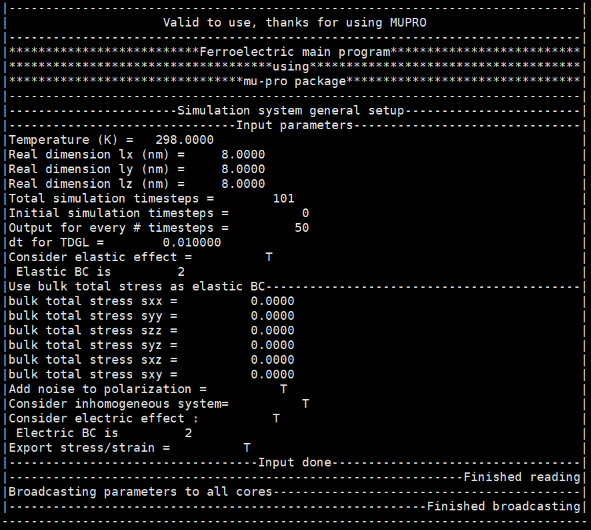
\includegraphics[]{img/quick-example-screen-output.PNG}

\caption{Example screen output}
\label{fig:quick-example-screen-output}
\end{figure}


After the program finished, you will get some output data files, all of which are in columnar pattern similar to the \textbf{Polar.in} file, that first three column define the position for data point, and then rest of the columns are data at each grid point. You may process the data or visualize it use the tools you're most familiar with.

We have provided several examples in out \muferro distributions including this quick tutorial files, but in the future when you are supposed to prepare these files yourself. It may be a daunting task for beginners, that's why we have this manual and some other tools to help you out.

For the creating the \textbf{input.in} file, you should refer to the Chapter \ref{chapter:input} and find the keyword you need for your specific case. For the \textbf{Polar.in} file, we prepared a small program called "Structure-Generator" that will help you create some commonly used or geometrically simple domain structures. And lastly, for the \textbf{pot.in} file, we are building an online database for phenomenological thermodynamic parameters, in the future you may want to download potential files from the website directly. For now, we put the thermodynamic parameters for some common materials in the "potentials" folder in the ferroelectric directory of \muferro distribution. But of course, you can use your own parameters for the potential file. The \textbf{pot.in} file is in the JSON format, you are allowed to change the value (number or string after the colon), but not the keys (the string before the colon, which is the name for the parameter we used in our simulation). Once the keys are changed, we can no longer find all of the value needed for simulation, and the program may crash. 

The post processing can also be quite challenging sometimes. We also prepare some gnuplot scripts, as well as a visualization GUI based on VTK+Qt to help you get started with the process. When you have more sophisticated visualization needs, you may find the right one that suits you the most.


\section{Structure of \muferro package}

\muferro is a Fortran 90 program. It allows for dynamic memory allocation and a single executable which can be used for any type of calculation. Generally the executables and the thermodynamic potentials should reside in the following directories: 


 \begin{forest}
      for tree={
        font=\ttfamily,
        grow'=0,
        child anchor=west,
        parent anchor=south,
        anchor=west,
        calign=first,
        inner xsep=7pt,
        edge path={
          \noexpand\path [draw, \forestoption{edge}]
          (!u.south west) +(7.5pt,0) |- (.child anchor) pic {folder} \forestoption{edge label};
        },
        % style for your file node 
        file/.style={edge path={\noexpand\path [draw, \forestoption{edge}]
          (!u.south west) +(7.5pt,0) |- (.child anchor) \forestoption{edge label};},
          inner xsep=2pt,font=\small\ttfamily
                     },
        before typesetting nodes={
          if n=1
            {insert before={[,phantom]}}
            {}
        },
        fit=band,
        before computing xy={l=15pt},
      }  
    [MuPro root directory
    %   [license.lic,file]
      [MUPRO\_1.0.6
        [Ferroelectric
            [{\color{green}Ferroelectric.exe},file]
            [Ferroelectric.pbs,file]
            [Potential]
            [Example]
        ]
        [Plot
            [Some gnuplot scripts ...,file]
            [Some bash scripts ...,file]
        ]
        [Structure-Generator
            [{\color{green}structureGenerator.exe},file]
            [Example]
        ]
      ] 
    ]
 \end{forest}


The \textbf{\mupro root directory} contains the license.lic file and the \mupro distribution of specific version, in this example is \textbf{MUPRO\_1.0.6}. In the \textbf{MUPRO\_1.0.6} folder there are three directories,
\begin{itemize}
\item[{\color{blue}Ferroelectric}] contains the main program for \muferro phase-field simulation, an example PBS script for you to submit jobs on systems using PBS job queue system, a \textbf{Potentials} folder which contains several commonly used thermodynamic potentials and physical properties that the program needs, and an \textbf{Example} folder that contains some example projects for you to try out and gain experience with using the program.
\item[{\color{blue}Plot}] contains three pairs of gnuplot script and bash script, one for 1D plot, one for 2D scalar heat plot, and the third for 2D vector glyph plot.
\item[{\color{blue}Structure-Generator}] contains a tool we prepared for you to generator some simple domain structures that can be directly used as the \textbf{Polar.in} file for \muferro program.
\end{itemize}


\chapter{Files of \muferro}

\section{Input files}

The following input files need to be presented in your working directory.
\begin{enumerate}
    \item input.in
    \item pot.in
    \item Polar.in
\end{enumerate}

Some other optional input files are

\begin{itemize}
    \item OctaTilt.in
    \item AFMtip.in
\end{itemize}

\subsection{input.in}

input.in file is in a free-format structure, each line of the file is made up of several parts
\begin{enumerate}
    \item[{\color{blue}\textbf{identifier}}] The string that appears before "{\color{red}=}" in each line. Identifiers are keywords that \muferro used to link the corresponding parameters in the program with values that are set in the input file. According to the values to be set, the identifiers can be classified into four types: 1. logical switch 2. choice options 3. single value 4. array values.  
    \item[{\color{blue}\textbf{values}}] The values that appears after "{\color{red}=}" and before "\#" in each line. These are numbers, booleans or string  values related to the identifier.
    \item[{\color{blue}\textbf{comments}}] The string after "\#".
\end{enumerate}


\vspace{1cm}
Let's take a look at some examples of the four types of identifiers and their values.
\begin{itemize}
    \item[{\color{blue}\textbf{logical switch}}] All logical switch type of identifiers start with "L" representing logical type, and the acceptable values are either True or False.\\
    \textbf{Example:} LELAST = True \hspace{0.5cm}   \# Consider the elastic effect on ferroelectric system
    \item[{\color{blue}\textbf{choice options}}] All choice option type of identifiers start with "C" representing choice, and the acceptable values are integers.\\
    \textbf{Example:} CELASBC = 2 \hspace{0.5cm} \# Set the elastic boundary condition to be stress free for bulk simulations.
    \item[{\color{blue}\textbf{single value}}] This type of identifiers only accept one value, and it can be either real or integer number depending on the specific identifier.\\
    \textbf{Example:} TIMESTEP = 10000 \hspace{0.5cm} \# Set the maximum simulation steps to be 10000.
    \item[{\color{blue}\textbf{array value}}] This type of identifiers accept more than one values, and it can be either real or integer number depending on the specific identifier.\\
    \textbf{Example:} SYSDIM = 128 128 40 \hspace{0.5cm} \# Set the simulation system size in x, y, z direction
\end{itemize}
Note that although identifiers in input.in are designed to be case insensitive, it is highly recommended to use all capitalized letters for IDENTIFIERS for clarity. 

\subsection{pot.in}

Like most materials simulation methods, phase field simulation for ferroelectrics require an potential, i.e., the Landau potentials of ferroelectric materials. The standard potential files are provided in the potentials folder of \muferro distribution. If missing, one can easily obtained the potentials files from online database. 


\begin{lstlisting}[style=json]
{
    "name"       : "BiTiO3",
    "Comment"       : "Fitted by Jian Jun Wang, the landau coefficient needs to be updated according to stress for every time step",
    "Reference"     : "JAP 108. 114105 (2010)",
    "CurieT"        : 390,
    "a0"            : 42769496,
    "p0"            : 0.26,
    "Landau"    :
        {   "a1"    : "5*10^5*160*(cosh(160/tem)/sinh(160/tem)-cosh(160/390)/sinh(160/390))",
            "a11"   : -1.154E8,
            "a12"   :  6.530E8,
            "a111"  : -2.105E9,
            "a112"  :  4.091E9,
            "a123"  : -6.688E9,
            "a1111" :  7.590E10,
            "a1112" : -2.193E10,
            "a1122" : -2.221E10,
            "a1123" :  2.416E10
        },
    "Electrostrictive"  :
        {
            "Q11"   :  0.11  ,
            "Q12"   : -0.045 ,
            "Q44"   :  0.029
        },
    "ElasticModulus"    :
        {
            "C11"   :  1.7794E11,
            "C12"   :  0.9635E11,
            "C44"   :  1.2199E11
        },
    "ElasticCompliance" :
        {
            "S11"   :  9.07E-12,
            "S12"   : -3.186E-12,
            "S44"   :  8.197E-12
        },
    "Gradient"          :
        {
            "G11"   : 5.10E-10,
            "G12"   : 0.0,
            "G44"   : 1.0E-11,
            "GM44"  : 1.0E-11
        }
}
\end{lstlisting}

\subsection{Polar.in} 

Polar.in is also a mandatory input file (or \muferro will start from a random noise of polarization). It stores the initial spatial distribution of polarization for calculation. It has a header line, specifing the total grid size of the system. The rest of the lines are made up of 9 columns, first three are data point positions, 4- to 6-th columns are polarization under global coordinate (the lab coordinate), 7- to 9-th columns are polarization in local coordinate (the crystal lattice coordinate). Be careful that the sequence of data point is z,y,x rather than x,y,z, that is to say, the data position gets update along z direction first, then y direction and in the last x direction. 

\begin{table}[h]
\centering
\caption{Example of Polar.in file}
\label{my-label}
\begin{tabular}{lllllllll}
10  & 10 & 10 &          &            &          &          &          &          \\
1   & 1  & 1  & 0.00E+00 & 0.00E+00 & 0.26E+00 & 0.00E+00 & 0.00E+00 & 0.26E+00 \\
1   & 1  & 2  & 0.00E+00 & 0.00E+00 & 0.26E+00 & 0.00E+00 & 0.00E+00 & 0.26E+00 \\
1   & 1  & 3  & 0.00E+00 & 0.00E+00 & 0.26E+00 & 0.00E+00 & 0.00E+00 & 0.26E+00 \\
... &    &    &          &            &          &          &          &          \\
1   & 1  & 10 & 0.00E+00 & 0.00E+00 & 0.26E+00 & 0.00E+00 & 0.00E+00 & 0.26E+00 \\
1   & 2  & 1  & 0.00E+00 & 0.00E+00 & 0.26E+00 & 0.00E+00 & 0.00E+00 & 0.26E+00 \\
1   & 2  & 2  & 0.00E+00 & 0.00E+00 & 0.26E+00 & 0.00E+00 & 0.00E+00 & 0.26E+00 \\
... &    &    &          &            &          &          &          &          \\
1   & 10 & 10 & 0.00E+00 & 0.00E+00 & 0.26E+00 & 0.00E+00 & 0.00E+00 & 0.26E+00 \\
2   & 10 & 10 & 0.00E+00 & 0.00E+00 & 0.26E+00 & 0.00E+00 & 0.00E+00 & 0.26E+00 \\
3   & 10 & 10 & 0.00E+00 & 0.00E+00 & 0.26E+00 & 0.00E+00 & 0.00E+00 & 0.26E+00 \\
... &    &    &          &            &          &          &          &          \\
10  & 10 & 10 & 0.00E+00 & 0.00E+00 & 0.26E+00 & 0.00E+00 & 0.00E+00 & 0.26E+00
\end{tabular}
\end{table}


\subsection{OctaTilt.in}

This file is similar to Polar.in, but stores the oxygen octahedral rotation around the three crystal axis. Please read this reference \cite{xue2014orientations} for more information about how we consider oxygen octahedral rotation in phase-field simulation. 

\subsection{AFMtip.in}
\label{sec:afm-tip}
This file is used to set the elastic/electric boundary conditions of ferroelectric films by an AFM tip as a mechanical indenter or as a bias electrode. The first line of this file contains three values, the first one is the times of changes of AFMP tip for the whole simulation, the second value is the choice of electric boundary condition, and the third value is the choice of elastic boundary condition, the meaning of different value for boundary condition can be found the in Chapter \ref{chapter:input} for identifier of \textbf{CTIPFORC} and \textbf{CTIPBIAS}.

The rest of \textbf{AFMtip.in} file are made up of 7 columns,
\begin{itemize}
    \item[{\color{blue}\textbf{timestep}}] timestep that the tip parameters get changed.
    \item[{\color{blue}\textbf{ntipx}}] grid position of the tip in x direciton.
    \item[{\color{blue}\textbf{ntipy}}] grid position of the tip in y direction.
    \item[{\color{blue}\textbf{bias}}] the electric potential applied to the tip.
    \item[{\color{blue}\textbf{force}}] the force applied by the tip to the film.
    \item[{\color{blue}\textbf{fricx}}] friction factor in x direction.
    \item[{\color{blue}\textbf{fricy}}] friction factor in y direction.
\end{itemize}


As an example, to simulate a moving AFM tip with 1V bias which writes along the path of the letter "P", one can prepare the AFMtip.in as 

\begin{lstlisting}[language=bash,caption={PBS script}]
        25    1    0
# timestep  ntipx  ntipy   bias  force fricx fricy
         1  30.00  90.00   1.00   0.00  0.0  0.0
      2001  30.00  84.00   1.00   0.00  0.0  0.0
      4001  30.00  78.00   1.00   0.00  0.0  0.0
      6001  30.00  72.00   1.00   0.00  0.0  0.0
      8001  30.00  66.00   1.00   0.00  0.0  0.0
     10001  30.00  60.00   1.00   0.00  0.0  0.0
     12001  30.00  54.00   1.00   0.00  0.0  0.0
     14001  30.00  48.00   1.00   0.00  0.0  0.0
     16001  30.00  42.00   1.00   0.00  0.0  0.0
     18001  30.00  36.00   1.00   0.00  0.0  0.0
     20001  30.00  90.00   1.00   0.00  0.0  0.0
     22001  36.00  90.00   1.00   0.00  0.0  0.0
     24001  42.00  90.00   1.00   0.00  0.0  0.0
     26001  48.00  90.00   1.00   0.00  0.0  0.0
     28001  54.00  90.00   1.00   0.00  0.0  0.0
     30001  60.00  90.00   1.00   0.00  0.0  0.0
     32001  60.00  84.00   1.00   0.00  0.0  0.0
     34001  60.00  78.00   1.00   0.00  0.0  0.0
     36001  60.00  72.00   1.00   0.00  0.0  0.0
     38001  60.00  66.00   1.00   0.00  0.0  0.0
     40001  60.00  60.00   1.00   0.00  0.0  0.0
     42001  54.00  60.00   1.00   0.00  0.0  0.0
     44001  48.00  60.00   1.00   0.00  0.0  0.0
     46001  42.00  60.00   1.00   0.00  0.0  0.0
     48001  36.00  60.00   1.00   0.00  0.0  0.0
\end{lstlisting} 

Notice the potential and force applied by tip is actually a distribution rather than uniform value. The value specified here is just one parameter used to get the distribution, you should always check the electric potential distribution and stress distribution to confirm that you get what you're expecting.

% Add the options of bias and force shapes here %

\section{Output files}
\label{sec:output-file}
All output files generated by \muferro are listed in Table 3.2\ref{tb:output-file-list}. They can be controlled by corresponding tags. Most of the output data files are time dependent, that is, the spatial distribution of some value at a given timestep. The file name for these time dependent data have one thing in common, they are all made up of three parts separated by "{\color{red}.}", the first one is the file name, such as "Polar", "Strain", the second one is the time step this data get output, which has a length of 8 digits, filled with 0 if the number length is less than 8, the third one is the file extension "dat". All possible data files are listed and explained in the Table \ref{tb:output-file-list}.

% Please add the following required packages to your document preamble:
% \usepackage{booktabs}
% \usepackage{graphicx}

\begin{table}[]
\centering
\caption{Output file list}
\label{tb:output-file-list}
\resizebox{\textwidth}{!}{%
\begin{tabular}{@{}rccl@{}}
\toprule
\textbf{File name}&\textbf{control} & \textbf{Columns} & \textbf{Explanation}                                                                       \\ \midrule
Polar             &     -    & 6                & Polarization in global coordinate and local coordinate                                     \\
Grade\_En         & LOUTGRAD & 1                & Gradient energy distribution                                                               \\
Grad\_For         & LOUTGRAD & 3                & Gradient driving force for polarization x, y, z                                            \\
Eigen\_Str        & LOUTELAS & 6                & Eigen strain distribution in voigt notation                                                \\
Strain            & LOUTELAS & 6                & Total strain distribution in voigt notation                                                \\
Elast\_Str        & LOUTELAS & 6                & Elastic strain distribution in voigt notation                                              \\
Stress            & LOUTELAS & 6                & Stress distribution in voigt notation                                                      \\
Displace          & LOUTELAS & 3                & Displacement x, y, z                                                                       \\
Elast\_En         & LOUTELAS & 1                & Elastic energy                                                                             \\
Elas\_For         & LOUTELAS & 3                & Elastic driving force for polarization x, y, z                                             \\
Elect\_En         & LOUTELEC & 1                & Electric energy                                                                            \\
Elefield          & LOUTELEC & 3                & Electric field x, y, z                                                                     \\
Elec\_Phi         & LOUTELEC & 1                & Electric potential                                                                         \\
Elec\_For         & LOUTELEC & 3                & Electric driving force x, y, z                                                             \\
Charges           & LOUTELEC & 3                & Bound charge, free charge, total charge                                                    \\
LandP\_En         & LOUTLAND & 1                & Landau energy for polarization as order parameter                                          \\
LandPFor          & LOUTLAND & 3                & Landau driving force for polarization x, y, z                                              \\
Eflexo            & LOUTFLEX & 3                & Flexoelectric driving force, as known as the effective electric field, x, y, z             \\
Gen\_ForX         & LOUTFORC & 6                & Elastic, electric, flexoelectric, landau, gradient and total driving force in x direction  \\
Gen\_ForY         & LOUTFORC & 6                & Elastic, electric, flexoelectric, landau, gradient and total driving force in y direction  \\
Gen\_ForZ         & LOUTFORC & 6                & Elastic, electric, flexoelectric, landau, gradient and total driving force in z direction  \\
OctaTilt          &     -    & 6                & Oxygen octahedral tilt around x, y, z axis                                                 \\
ElasQFor          & LOUTELAS & 3                & Elastic driving force for oxygen octahedral tilt                                           \\
GradQ\_En         & LOUTGRAD & 1                & Gradient energy of oxygen octahedral tilt                                                  \\
GradQFor          & LOUTGRAD & 3                & Gradient driving force for oxygen octahedral tilt x, y, z component                        \\
LandQ\_En         & LOUTLAND & 1                & Landau energy of oxygen octahedral tilt as order parameter                                 \\
LandQFor          & LOUTLAND & 3                & Landau driving force for oxygen octahedral tilt                                            \\
GenQForX          & LOUTFORC & 4                & Elastic, landau, gradient and total driving force for oxygen octahedral tilt in x axis \\
GenQForY          & LOUTFORC & 4                & Elastic, landau, gradient and total driving force for oxygen octahedral tilt in y axis \\
GenQForZ          & LOUTFORC & 4                & Elastic, landau, gradient and total driving force for oxygen octahedral tilt in z axis \\ \bottomrule
\end{tabular}%
}
\end{table}



\section{Pre-processing files}

\subsection{PBS file for submitting tasks}
Many of the linux high performance computing system are using "Portable Batch System (PBS)" to manage the queueing and allocation of jobs on the cluster. For these types of systems, a PBS script is needed for job submission.

\begin{lstlisting}[language=bash,caption={PBS script}]
#PBS -l nodes=1:ppn=2
#PBS -l walltime=24:00:00 
#PBS -N Ferroelectric 
#PBS -j oe
#PBS -A allocation_to_use
#PBS -M myemail@school.edu
#PBS -m ae

cd $PBS_O_WORKDIR 
echo `date` 
mpirun MUPRO -ferroelectric.exe 
echo `date` 
\end{lstlisting}


\subsection{scripts for batch tasks}
From time to time you may want to run a series of jobs to see the trend of how things change. The following script gives an example that replace custom keyword in the input.in file, \textbf{nx\_size} and \textbf{lx\_size}, with different numbers ranging from 40 to 120, before submitting the job with PBS command. Note that the keyword used here for batch substitution should not be the same as the identifiers (left side of "=") specified in input.in.  

\begin{lstlisting}[language=bash,caption={Batch submission of jobs}]
#! /bin/bash

length=( 40 60 80 100 120 )

for interval in "${length[@]}"
do
    let nx=$interval
    let lx=($nx)
    mkdir $interval
    cd $interval
    cp ../input.in .
    sed -i "s/nx_size/${nx}/g" input.in 
    sed -i "s/lx_size/${lx}/g" input.in 
    qsub ferro.pbs
    cd ..
done

\end{lstlisting}

% May be not provide these two functions here 
% \subsection{Microstructure generator} 

% \subsection{AFMtip generator} 

\section{Post-processing files}
\subsection{GNUPlot \& bash scripts}

In the \textbf{Plot} folder we provide several script that enables you to quickly draw some 1D plot, 2D scalar plot and 2D vector plot for the output data \muferro program generated.

\subsubsection{plot\_1d.sh}

This script helps you to draw 1D profile of a one column vs another in the data file. It takes at least 9 arguements: 1. minimum value in x direction, 2. maximum value in x direction, 3. minimum value in y direction, 4. maximum value in y direction, 5. minimum value in z direction, 6. maximum value in z direction, 7. column number of the data used for the horizontal axis of the 1D plot, 8. column number of the data used for the vertical axis of the 1D plot, 9. name of the data file.

You can actually pass more data file names as additional arguments, and the script will draw the same 1D profile for all of the data files on one figure.

An example usage of the script is shown in Listing \ref{lst:1d-plot-example}. It means slice the \textbf{Polar.00001000.dat} file into one line, $1\leq x \leq 128$, and $y=40, z=20$, then plot the figure using the first column and the fourth column of the data file, which correspond to grid position in x direction and the x component of polarization in global coordinates. The output figure has a default name of \textbf{fig1d.png}.

\begin{lstlisting}[caption={Example of 1D plot usage.},label={lst:1d-plot-example}]
plot_1d.sh 1 128 40 40 20 20 1 4 Polar.00001000.dat
\end{lstlisting}


\subsubsection{plot\_2ds.sh}
This script helps you to draw 2D heat plot for one column in the data file. It takes at 7 arguements: 1. minimum value in x direction, 2. maximum value in x direction, 3. minimum value in y direction, 4. maximum value in y direction, 5. minimum value in z direction, 6. maximum value in z direction, 7. column number of the data you want to use for the heat plot.

An example usage of the script is shown in Listing \ref{lst:2d-plot-scalar-example}. It means slice the \textbf{Polar.00001000.dat} file into one plane, $1\leq x \leq 128, 1\leq y \leq 128$, and $z=20$, then plot the figure using the fourth column of the data file, which correspond to the x component of polarization in global coordinates. The output figure has a default name of \textbf{fig2ds\_Polar.00001000.png}.

\begin{lstlisting}[caption={Example of 2D scalar plot usage.},label={lst:2d-plot-scalar-example}]
plot_2ds.sh 1 128 1 128 20 20 4 Polar.00001000.dat
\end{lstlisting}

\subsubsection{plot\_2dv.sh}
This script helps you to draw 2D vector plot for two column in the data file. The 3D vectors are projected to the 2D slice you specify. It takes at least 8 arguements: 1. minimum value in x direction, 2. maximum value in x direction, 3. minimum value in y direction, 4. maximum value in y direction, 5. minimum value in z direction, 6. maximum value in z direction, 7. choice between global and local coordinates (1-global, 2-local) of the vector to be drawn, 8. column number according to which the vectors are colored.

An example usage of the script is shown in Listing \ref{lst:2d-plot-vector-example}. It means slice the \textbf{Polar.00001000.dat} file into one plane, $1\leq x \leq 128, 1\leq y \leq 128$, and $z=20$, and global coordiantes, then plot the figure using the fourth and fifth columns of the data file, which correspond to the x and y component of polarization in global coordinates, px is used as the x component of the 2D vector and py as the y component. And the vector will be colored according to the 5-th column, which is the y-components of vectors. The output figure has a default name of \textbf{fig2dv\_Polar.00001000.png}.

\begin{lstlisting}[caption={Example of 2D vector plot usage.},label={lst:2d-plot-vector-example}]
plot_2dv.sh 1 128 1 128 20 20 1 4 Polar.00001000.dat
\end{lstlisting}

% 4. cut.sh

% Extract a box section from the output files. 

% 5. interp.f90 

% Linear interpolation of output data points for better figure illustration. Not encouraged. 

% 6. expand2D.f90 / expand3D.f90

% Extend output files laterally or 3-dimensionally. 


\chapter{The input.in File}
\label{chapter:input}

\section{List of most important parameters}

\setlength{\LTleft}{-0.7in}
\setlength{\LTright}{0in}
\begin{longtable}{p{0.15\textwidth} p{0.15\textwidth} p{0.1\textwidth} p{0.32\textwidth} p{0.35\textwidth}}

\caption{Most important tags used for \muferro} % needs to go inside longtable environment
\label{tab:myfirstlongtable}

\cr     & \textbf{Tags} & \textbf{Class} & \textbf{Default} & \textbf{Description} \\ \hline
\multirow{5}{*}{\textbf{System}} & SYSDIM & Vector & 10, 10, 10 & Grid points in x, y, z \\ \cline{2-5}
 & REALDIM & Vector & Same as SYSDIM & Real length along x, y, z \\ \cline{2-5} 
 & SUBTHICK & Scalar & 0 & Grid points for substrate thickness \\ \cline{2-5} 
 & FILMTHICK & Vector & 0 & Grid points for film thickness \\ \cline{2-5} 
 & ROTANGLE & Vector & 0.0, 0.0, 0.0 & Euler rotation angle around z, $x'$, $z''$ \\ \hline
\multirow{4}{*}{\textbf{Time}} & TTOTAL & Scalar & 1000 & Total timesteps \\ \cline{2-5} 
 & TSTART & Scalar & 0 & Initial timestep \\ \cline{2-5} 
 & TOUT & Scalar & 200 & Time interval for output \\ \cline{2-5} 
 & TDELTA & Scalar & 0.01 & Delta t of TDGL \\ \hline
\multirow{2}{*}{\textbf{Solvers}} & LINHOM & Flag & FALSE & Flag for inhomogeneous solver \\ \cline{2-5} 
 & CDER & Choice & \begin{tabular}[c]{@{}l@{}}0- step-corrected FFT\\ 1- FDM\\ 2- normal FFT\end{tabular} & Choices of derivative solver \\ \hline
\textbf{Thermal} & TEM & Scalar & 298.0 & Temperature in Kelvin \\ \hline
\multirow{5}{*}{\textbf{Polarization}} & CPOLARBC & Choice & \begin{tabular}[c]{@{}l@{}}0- natural BC\\ 1- free BC\\ 2- blocked BC\\ 3- small extrapolation length\\ 4- zero bound charge\\ 5- large extrapolation length\end{tabular} & Choices of boundary condition,for Px, Py, Pz \\ \cline{2-5} 
 & ETRLP & Vector & 0.0, 0.0, 0.0 & Extrapolation length of Px, Py, Pz in nm \\ \cline{2-5} 
 & LPNOISE & Flag & FALSE & Flag of polarization noise \\ \cline{2-5} 
 & PNOISMAG & Scalar & 0.1 & Magnitude of polarization noise \\ \cline{2-5} 
 & PNOISEED & Scalar & 10 & Seed of polarization noise \\ \hline
\multirow{6}{*}{\textbf{Elastic}} & LELAS & Flag & TRUE & Flag of elastic energy \\ \cline{2-5} 
 & CELASBC & Choice & \begin{tabular}[c]{@{}l@{}}0- film\\ 1- bulk strain\\ 2- bulk stress\end{tabular} & Choices of elastic boundary conditions \\ \cline{2-5} 
 & MISFIT & Vector & 0.0, 0.0, 0.0 & Misfit strain exx, eyy, exy \\ \cline{2-5} 
 & STRAIN & Vector & 0.0, 0.0, 0.0, 0.0, 0.0, 0.0 & Strain BC for bulk, exx, eyy, ezz, eyz, ezx, exy \\ \cline{2-5} 
 & STRESS & Vector & 0.0, 0.0, 0.0, 0.0, 0.0, 0.0 & Stress BC for bulk, sxx, syy, szz, syz, szx, sxy \\ \cline{2-5} 
 & TIPRAD & Scalar & 50.0 & Tip radius in nm \\ \hline
\multirow{5}{*}{\textbf{Electric}} & LELEC & Flag & TRUE & Flag of electric energy \\ \cline{2-5} 
 & CELECBC & Choice & \begin{tabular}[c]{@{}l@{}}1- open circuit\\ 2- short circuit\\ 3- top open bottom short\\ 4- top short bottom open\\ 5- bulk\end{tabular} & Choices of electric boundary conditions \\ \cline{2-5} 
 & TIPGAMMA & Scalar & 10.0 & Lortenz $gamma$ for tip in nm \\ \cline{2-5} 
 & SCRBOT & Scalar & 0.0 & Screening factor of bottom electrode \\ \cline{2-5} 
 & SCRTOP & Scalar & 0.0 & Screening factor of top electrode \\ \hline
\textbf{Gradient} & GRADCON & Vector & 0.6, 0.0, 0.3 & Gradient energy tensor component g11, g12 and g44 \\ \hline
\multirow{2}{*}{\textbf{Flexoelectric}} & LFLEXO & Flag & FALSE & Flag of flexoelectric energy \\ \cline{2-5} 
 & FLEXOCON & Vector & 5.1, 3.3, 0.045 & Flexoelectric tensor component f11, f12, and f44 \\ \hline
\multirow{5}{*}{\textbf{\begin{tabular}[c]{@{}c@{}}Oxygen \\ Octahedral \\ Rotation\end{tabular}}} & LOCTILT & Flag & FALSE & Flag of oxygen octahedral tilt \\ \cline{2-5} 
 & GRADQCON & Vector & 1.0 0.0 0.5 & Gradient energy tensor of OOT component v11, v12, v44 \\ \cline{2-5} 
 & LQNOISE & Flag & FALSE & Flag of OOT noise \\ \cline{2-5} 
 & QNOISMAG & Scalar & 0.1 & Magnitude of OOT noise \\ \cline{2-5} 
 & QNOISEED & Scalar & 10 & Seed of  OOT noise \\ \hline
\multirow{6}{*}{\textbf{Outputs}} & LOUTLAND & Flag & FALSE & Flag of output Landau energy of polarization \\ \cline{2-5} 
 & LOUTELAS & Flag & FALSE & Flag of output elastic energy \\ \cline{2-5} 
 & LOUTELEC & Flag & FALSE & Flag of output elastic energy \\ \cline{2-5} 
 & LOUTGRAD & Flag & FALSE & Flag of output gradient energy \\ \cline{2-5} 
 & LOUTFLEX & Flag & FALSE & Flag of output flexoelectric fields \\ \cline{2-5} 
 & LOUTFORC & Flag & FALSE & Flag of output driving forces \\ \hline


\end{longtable}
%\end{table}


\begin{parameter}{CDER}{choice derivative}{choice}


\begin{option}
\item[{\color{blue}0}] FFT method with step correction 
\item[1] finite difference method 
\item[2] FFT method without step correction 
\end{option}

\noindent\describe
Choose the numerical methods for taking derivatives. The places may be affected by this option include bound charges (divergence of polarization), elecric field (gradient of electric potential), and flexoelectric field/flexoelectric driving force(derivatives of stress tensors)


\noindent\notes
Do not change CDER unless following situations:

1. Flexofield calculations
\end{parameter}





\begin{parameter}{CELASBC}{choice elastic boundary conditions}{Choice}


\begin{option}
\item[0] film boundary condition, i.e., stress-free at film surface and clamped at film bottom. (for detailed treatment please refer to micromechanics [Li 2002][Khachaturyan Chap 8?])
\item[1]strained boundary condition for bulk, i.e., clamped boundary condition. Assign a fixed strain tensor as average strain value of bulk system. Use this combined with \textbf{STRAIN}-tag [Ref]. 
\item[{\color{blue}2}]stressed boundary condition for bulk. Assign a fixed stress tensor as average stress value of bulk system. Use this combined with \textbf{STRESS}-tag [Ref]. 


\end{option}

\describe
Choose the elastic boundary condition when solving for mechanical equilibrium.

\notes
\noindent
\begin{enumerate}
    \item CELASBC = 1 and 2 only work for bulk system while CELASBC = 0 only works for film system. Please be consistent with the \textbf{LBULK} tag. 
    \item CELASBC = 1 is related to \textbf{STRAIN}\\   
CELASBC = 2 is related to \textbf{STRESS}\\
CELASBC = 0 is related to \textbf{MISFIT} 
\end{enumerate}

\end{parameter}

\begin{parameter}{CELECBC}{Choice electric boundary conditions}{Choice}
\begin{option}
\item[{\color{blue}0}]bulk boundary condition, i.e., given a fixed electric field to bulk system. Specify applied electric field by ELECFIELD.
\item[1] open-circuit boundary conditions at film surface and bottom.
\item[2] short-circuit boundary condition at film surface and bottom.
\item[3] open-circuit boundary condition at film surface while short-circuit boundary condition at film bottom.
\item[4] open-circuit boundary condition at film bottom while short-circuit boundary condition at film surface.
\end{option}

\describe
Choose the electric boundary condition of electrostatic equation

\notes
\begin{enumerate}
    \item CELECBC  =  0  only  works  for  bulk  systems  while  other  options  only  work  for  filmsystems.
    \item CELECBC = 0 is paired with ELECFIELD.
    \item In experiment, even without electrode, there are still plenty of mechanisms that can compensate charges at the interface or surface, so be careful when to use the open circuit condition.
\end{enumerate}

\end{parameter}


\begin{parameter}{CPOLARBC}{Choice polarization boundary conditions}{Choice}
\begin{option}
\item[0]natural boundary condition 
\item[{\color{blue}1}] Neumann boundary condition, $\frac{dP}{dz} = 0$ at film surface and bottom.
\item[2] Dirichlet boundary condition, $P = 0$ at film surface and bottom.
\end{option}

\describe
Choose the boundary condition for polarization when evolving the time dependent Ginzburg Landau equation. The polarization boundary condition is related to extrapolation length in journal articles.

\notes
The boundary condition for polarization is a value that is difficult to determine, for normal calculation that focus on domain structures, you can go with the default Neumann boundary condition, which set derivative to zero. Only when you're simulating some special distribution near the interface or surface, you may want to try the other two boundary conditions.
\end{parameter}


\begin{parameter}{DIELECON }{Dielectric constants (background) }{Vector, Real}

\describe
To set background dielectric constant which will override the dielectric constants assigned in the pot.in file. 

\notes
\begin{enumerate}
    \item The background dielectric constant denotes the dielectric response to applied electric field apart from the spontaneous polarization. It also represents the dielectric constant at infinite high temperature in the plot of dielectric permittivity as a function of temperature. For detailed description, please refer to [Ref. Tagantsev, Zheng \& Woo]
\end{enumerate}



\end{parameter}


\begin{parameter}{ELECFIELD}{Electric Field}{Vector, Real}  

\describe
This tag sets up the electric boundary condition of bulk system using an applied electric field. It can be used to obtain the PE loop of a bulk system. Three real numbers must be specified for this tag, electric field along x, y and z direction, separated by space.

\notes
\begin{enumerate}
    \item The unit of assigned electric field is in V/m.
\end{enumerate}

\end{parameter}


% \begin{parameter}{ETRLP}{Extrapolation length of polarization}{Vector} 
% \describe
% The extrapolation length describes the surface effect on spontaneous polarization in ferroelectrics. It is defined as $\lambda$ in $P + \frac{1}{\lambda} \frac{dP}{dz} = 0$. 

% \notes
% \end{parameter}

\begin{parameter}{FILMTHICK}{Film thickness}{Integer} 
\describe
Film thickness is the number of simulation grid points for the film. Related value is \textbf{SUBTHICK}, which is the number of simulation grid for the substrate. When the film thickness is set to 0, then the program will treat the system as a bulk simulation with periodic boundary condition in all three directions rather than a thin film simulation which is only periodic in the in-plane (x,y) direction.

\notes 
\begin{enumerate}
    \item Set to 0 for bulk system, non 0 for thin film system.
\end{enumerate}
\end{parameter}

\begin{parameter}{FLEXOCON}{Flexoelectric constants}{Vector,real} 

\describe
This vector tag sets the three independent flexoelectric constants of cubic symmetry material, i.e., longitudinal f1111, transverse f1122, shear f1221. 

\notes
\begin{enumerate}
    \item The unit of assigned flexoelectric constant is in V.
    \item The theoretical estimation of flexoelectric constant for perovskites is within 0~20 V. The sign is usually not determined. 
\end{enumerate}

\end{parameter}


\begin{parameter}{FRACTION}{Material composition fraction}{Scalar,real} 

\describe
This tag set the fraction for materials such as PZT, PMNPT and KNN.  

\notes
\begin{enumerate}
    \item For Pb(Zr\textsubscript{1-x},Ti\textsubscript{x})O\textsubscript{3}, this value set the Ti fraction.
    \item For PMN-xPT, this value set the fraction of PT.
    \item For K\textsubscript{1-x}N\textsubscript{x}NbO\textsubscript{3}, this value set the Na fraction. 
\end{enumerate}

\end{parameter}


\begin{parameter}{GRADPCON}{Gradient energy constant of polarization}{Vector, real}
\describe
Gradient coefficient for polarization. Specifying this value will override the default one obtained from pot.in file. Different from the value used in pot.in, which is in SI unit, the value set by GRADPCON is in reduced unit normalized by $a_0l_0^2$, in which $a_0$ is chosen to be the value of $a_1$, the first coefficient for landau potential, at 298k, and $l_0$ is the denominator for length, for ferroelectric case we use $10^{-9}m$ per grid as its value. Three values need to be specified for tag, coefficient G11, G12 and G44, as in the formular for gradient energy
$\frac{G_{11}}{2}(P_{1,1}^2+P_{2,2}^2+P_{3,3}^2)+G_{12}(P_{1,1}P_{2,2}+P_{1,1}P_{3,3}+P_{3,3}P_{2,2})+\frac{G_{44}}{2}[(P_{1,2}+P_{2,1})^2+(P_{1,3}+P_{3,1})^2+(P_{3,2}+P_{2,3})^2]$ [Phenomenological model of a 90° domain wall in BaTiO3-type ferroelectrics]PHYSICAL REVIEW B 74, 104104 2006. The default value for gradient energy coefficient is $G_{11}=0.6$, $G_{12}=-0.6$ and $G_{44}= 0.6$. It is recommended to test the gradient energy coefficient value for your specific system, that the domain wall width should be more than 1.5 grid thick. 

\notes
\begin{enumerate}
    \item Default value for gradient energy coefficient is $G_{11}=0.6$, $G_{12}=-0.6$ and $G_{44}= 0.6$.
\end{enumerate}

\end{parameter}
\begin{parameter}{GRADQCON}{Gradient energy contant of oxygen octahedral rotation}{Vector, real} 

\describe
Gradient coefficient for oxygen octahedral rotation. Specifying this value will override the default one obtained from pot.in file. Different from the value used in pot.in, which is in SI unit, the value set by GRADQCON is in reduced unit normalized by $b_0l_0^2$, in which $b_0$ is chosen to be the value of $b_1$, the first coefficient for landau potential, at 298k, and $l_0$ is the denominator for length, for ferroelectric case we use $10^{-9}m$ per grid as its value. Three values need to be specified for tag, coefficient G11, G12 and G44, as in the formular for gradient energy
$\frac{v_{11}}{2}(q_{1,1}^2+q_{2,2}^2+q_{3,3}^2)+v_{12}(q_{1,1}q_{2,2}+q_{1,1}q_{3,3}+q_{3,3}q_{2,2})+\frac{v_{44}}{2}[(q_{1,2}+q_{2,1})^2+(q_{1,3}+q_{3,1})^2+(q_{3,2}+q_{2,3})^2]$. The default value for gradient energy coefficient is $v_{11}=1$, $v_{12}=-1$ and $v_{44}= 1$.  

\notes
\begin{enumerate}
    \item Default value for gradient energy coefficient is $v_{11}=1$, $v_{12}=-1$ and $v_{44}= 1$.
\end{enumerate}
\end{parameter}


\begin{parameter}{LAFMTIP}{Flag of AFM tip}{logic}
\describe
This flag controls whether to include an AFM tip (or time-variant electric bias for film systems) into the system or not. When turning on, it requires an extra input file, \textbf{AFMtip.in}, which specifies the moving paths, electric bias and mechanical load of an AFM tip. For the format of \textbf{AFMtip.in}, please refer to Section \ref{sec:afm-tip}.
\notes 

\end{parameter}

\begin{parameter}{LBULK}{Flag for bulk or thin film system}{logic}
\describe
This flag controls whether the simulated system is treated as a bulk or thin film one. This will affect several other tags, such electric and elastic boundary conditions. 

\notes 
For thin film system, you need to specify the \textbf{SUBTHICK} and \textbf{FILMTHICK}

\end{parameter}


\begin{parameter}{LELAS}{Flag of elasticity}{logic} 
\describe
This flag controls whether to consider the elastic effect or not. It is recommended to turn it on for normal ferroelectric simulations, since all ferroelectrics are ferroelastic materials, elastic effect plays a key role in determining the equilibrium domain structure. When LELAS is turned on, a mechanical equilibrium equation $\sigma_{ij,i}=0$ is solved using spectral method, and the elastic driving force for polarization can be obtained based on the calculated stress distribution. In the thin film cases, the boundary condition is periodic in the x-y (in-plane) direction, traction (stress components that are related to the z direction, $\sigma_{33}$, $\sigma_{13}$, $\sigma_{23}$) free for the film surface, and displacement free at the some distance into the substrate, and such distance is given by the \textbf{SUBTHICK}. In the bulk cases, average stress or strain can be specified.[yulan li 2002]

\notes

\end{parameter}

\begin{parameter}{LELEC}{Flag of electricity}{Logic} 
\describe
This flag controls whether to consider the electric effect or not. It is recommended to turn it on for all kinds of ferroelectric simulaitons, because electric field can have a significant influence on polarization. When turned on, a Poisson equation is solved using the spectral method. In the thin film case, there is periodic boundary condition in the in-plane (x-y) direction, and short or open circuit boundary condition for the film normal direction. In the bulk cases, the average electric field can be specified.[yulan li 2002]

\notes
\end{parameter}

\begin{parameter}{LFLEXO}{Flag of flexoelectricity}{Logic}
\describe
This flag controls whether to consider the flexoelectric effect or not. 

\notes
\end{parameter}


\begin{parameter}{LINHOM}{Flag of inhomogeneous system}{Logic}
\describe
This flag controls whether your want your simulated system to be considered as homogeneous or not. The homogeneous is not in the sense of different phases but in terms of material properties, such as elastic constant or dielectric constant. Inhomogeneous system require material properties to be set pointwise in the form of an array rather than a single constant, which will lead to significantly more memory usage. So only turn this flag on when necessary. 

\notes
\begin{enumerate}
    \item Only use this flag when necessary, it will significantly increase both the calculation time and memory usage.
\end{enumerate}
\end{parameter}


\begin{parameter}{LOCTILT}{Flag of oxygen octahedral rotation}{Logic} 
\describe
This flag controls whether you want to evolve the oxygen octahedral tilt/rotation in the simulation system. Oxygen octahedral tilt is a second set of order parameter, and it is coupled with elasticity and polarization. [Fei paper]

\notes
\end{parameter}
\begin{parameter}{LOUTELAS}{Flag of output elasticity}{Logic}
\describe
This flag controls whether output of elastic related data files are allowed. Files include \textbf{Displace}, \textbf{Eigen\_St}, \textbf{stress}, \textbf{strain}, \textbf{ElastEn}, \textbf{Elas\_For}, for more details, please see Section \ref{sec:output-file}.

\notes 
\end{parameter}
\begin{parameter}{LOUTELEC}{Flag of output electricity}{Logic} 
\describe
This flag controls whether output of electric related data files are allowed. Files include \textbf{Elefield},  \textbf{Elec\_Phi}, \textbf{Charges}, \textbf{Elec\_For}, for more details, please see Section \ref{sec:output-file}.

\notes 
\end{parameter}
\begin{parameter}{LOUTFLEX}{Flag of output flexoelectric field}{Logic} 

\describe
This flag controls whether output of flexoelectric are allowed. Files include \textbf{Eflexo}, for more details, please see Section \ref{sec:output-file}.

\notes
\end{parameter}

\begin{parameter}{LOUTFORC}{Flag of output all driving forces}{Logic} 
\describe
This flag controls whether output of driving force is allowed. Files include \textbf{Gen\_ForX}, \textbf{Gen\_ForY}, \textbf{Gen\_ForZ}, for more details, please see Section \ref{sec:output-file}.

\notes
\end{parameter}

\begin{parameter}{LOUTGRAD}{Flag of output gradient energy}{Logic} 
\describe
This flag controls whether output of gradient energy is allowed. Files include \textbf{Grade\_En}, \textbf{Grad\_For}, for more details, please see Section \ref{sec:output-file}.

\notes 

\end{parameter}

\begin{parameter}{LOUTLAND}{Flag of output Landau energy}{Logic} 
\describe
This flag controls whether output of landau energy is allowed. Files include \textbf{LandP\_En}, \textbf{LandPFor}, for more details, please see Section \ref{sec:output-file}.

\notes
\end{parameter}

\begin{parameter}{LPNOISE}{Flag of initial noise of polarization}{Logic} 
\describe
This flag controls whether initial noise for polarization is added or not. The noise is a uniform distribution generated using the fortran subroutine RANDOM. The random seed is set with \textbf{PNOISEED}.

\notes 
\end{parameter}


\begin{parameter}{LQNOISE}{Flag of initial noise of oxygen octahedral rotation}{Logic} 
\describe
This flag control whether initial noise for oxygen octahedral tilt is added or not. The noise is a uniform distribution generated using the fortran subroutine RANDOM. The random seed is set with \textbf{QNOISEED}.

\notes
\end{parameter}


\begin{parameter}{MISFIT}{Misfit strain}{Vector,real} 
\describe
Misfit strain that is due to the lattice mismatch between film and substrate, calculated by $\frac{a_s-a_f}{a_s}$, in which $a_s$ is the lattice parameter for substrate and $a_f$ is the lattice parameter for thin film. Three values need to set for this tag, they are ($\epsilon_{11}$ $\epsilon_{22}$ $\epsilon_{12}$).

\notes 
\end{parameter}

\begin{parameter}{PNOISEED}{Seed for polarization noise}{Integer} 
\describe
Set the seed value for the polarization noise generated with RANDOM subroutine. This is the value used in fortran subroutine RANDOM\_SEED

\notes
\end{parameter}

\begin{parameter}{PNOISMAG}{Noise magnitude for polarization}{Real}
\describe
Set the magnitude for polarization noise.

\notes
\end{parameter}

\begin{parameter}{QNOISEED}{Seed for oxygen octahedral rotation}{Integer}
\describe
Set the seed value for the oxygen octahedral rotation noise generated with random subroutine. This is the value used in fortran subroutine RANDOM\_SEED.

\notes:
\end{parameter}

\begin{parameter}{QNOISMAG}{Noise magnitude for oxygen octahedral rotation}{Real} 
\describe
Set the magnitude for oxygen octahedral rotation noise.

\notes:
\end{parameter}

\begin{parameter}{REALDIM}{Real dimension}{Vector, real}
\describe
REALDIM is a 3 dimension vector specifying the real size of the simulated system in x, y and z direction with an unit of nanometer. Different from the SYSDIM value, REALDIM is real number rather than integer. In order to get a more reasonable simulation result, it is recommended that the width of domain walls no thinner than 1.5 simulation grid point. In other word, if you know the domain wall thickness for your simulated system is 1.5 nm, then each grid point (set with SYSDIM) in your system should be fine representing 1 nm, leading to REALDIM=1nm*SYSDIM. 


\notes
\end{parameter}

\begin{parameter}{ROTANGLE}{Rotation Euler angles}{Vector}
\describe
Rotation angle determines the crystallography orientation of the material, it is a 3 dimensional vector of real number that correspond the the three euler angle. We used a very common proper euler angle, z-x-z,  which means first angle is the rotation around z axis, second angle is the rotation around y axis in the new coordinate system, and the third value is the rotation angle around z axis in the new system. 

\notes
\end{parameter}

\begin{parameter}{SCREENBOT}{Screening factor at film bottom}{Real}
\describe
This value is used for setting the screening percentage of film/substrate interface charges under open circuit electric boundary conditions. It can only be used for the thin film type of system, and for open circuit conditions, for which the electric displacement is fixed.

\notes
\end{parameter}

\begin{parameter}{SCREENTOP}{Screening factor at film top}{Real}
\describe
This value is used for setting the screening percentage of top surface charges under open circuit electric boundary conditions. It can only be used for the thin film type of system, and for open circuit conditions, for which the electric displacement is fixed.

\notes
\end{parameter}

\begin{parameter}{STRAIN}{Applied strain}{Vector, Real}
\describe
This value is a 6 dimension vector, ($\epsilon_{11}$, $\epsilon_{22}$, $\epsilon_{33}$, $\epsilon_{23}$, $\epsilon_{13}$, $\epsilon_{12}$), specifying the applied strain for bulk system.

\notes
\end{parameter}

\begin{parameter}{STRESS}{Applied stress}{Vector, Real} 
\describe
This value is a 6 dimension vector, ($\sigma_{11}$, $\sigma_{22}$, $\sigma_{33}$, $\sigma_{23}$, $\sigma_{13}$, $\sigma_{12}$), specifying the applied stress for bulk system.

\notes
\end{parameter}

\begin{parameter}{SUBTHICK}{Substrate thickness}{Scalar, integer} 
\describe
The integer value set the thickness of the substrate, which is only meaningful for the thin film case. The \textbf{SUBTHICK} is in terms of simulation grid point rather than in real world unit, such as nanometer. This value actually means the thickness of substrate lattice that is been distorted due to the mismatch between film and substrate material. And at such substrate thickness away from the interface, the no displacement, or fully clamped elastic boundary condition is applied. For example, if you set \textbf{SUBTHICK} to be 10, and in your simulation system 1 grid equals 1nm, then its physical meaning is you consider the substrate lattice not affected by the thin film, if deeper than 10 nm away from the interface. 

\notes
\end{parameter}

\begin{parameter}{SYSDIM}{System dimension}{Vector(3), real}
\describe
This 3 dimensional vector holds the dimension in x, y and z direction of the simulation system in real world unit of nanometer.

\notes
\end{parameter}

\begin{parameter}{TDELTA}{Increment time step}{Real}
\describe
This value controls the size of marching step when we evolve the TDGL equation to minimize total free energy. Larger timestep can leads to shorter simulation time, but may also easily leads to inconvergency. Recommended values are 0.01 or 0.02 .

\notes
\end{parameter}

\begin{parameter}{TEM}{Temperature}{Real}
\describe
The value set the current temperature of the simulation system. Default value is room temperature of 298k, since most experiments are carried out under such conditions.

\notes
\end{parameter}

\begin{parameter}{TIPGAMMA}{AFM tip gamma}{Real}
\describe
This value defines the gamma coefficient $\gamma$ in a Lorentz distribution to describe the electric potential distribution on top of the film surface, i.e., 
\begin{equation}
    \phi(x,y) = \frac{ \gamma^2 }{(x-x_{tip})^2+(y-y_{tip})^2+\gamma^2}
\end{equation}

\notes
\begin{enumerate}
    \item The unit of assigned gamma is in nm.
\end{enumerate}
\end{parameter}

\begin{parameter}{TIPRAD}{AFM tip radius}{Real}
\describe
This value defines the AFM tip radius (assuming spherical). Then the contact radius will be calculated according to Hertz contact model of a spherical indenter.\cite{Fischer-Cripps2000} 

\notes
\begin{enumerate}
    \item The unit of assigned tip radius is in nm. 
    \item The common value of a tip radius is around 30 - 100 nm. 
    \end{enumerate}
\end{parameter}

\begin{parameter}{TOUTPUT}{Interval timestep for output}{Integer} 

\describe
 This value set the interval for output all output data files in Secition \ref{sec:output-file}. 

\notes
\end{parameter}

\begin{parameter}{TSTART}{Start timestep}{Integer}
\describe
This value set the starting timestep of the simulation. Default value is 0, which is the case if you're running a new simulation. But when you are restarting from a previous output, then you may want to set this TSTART value to be where you stopped before, and then it won't create confusion in the naming of output data.

\notes
\end{parameter}

\begin{parameter}{TTOTAL}{Total timesteps}{Integer} 
\describe
This value set the total amount of timesteps that you want to run. For example, if the TSTART value is 10000, and the TTOTAL is 10000, then as long as you have enough wall time to finish the simulation, the program will stop at step 20000.

\notes
\end{parameter}

\clearpage{}

\chapter{Examples}
\section{Equilibrium domain structure of BaTiO\textsubscript{3} single crystal}

This example is about calculating the equilibrium domain structure for bulk single crystal BaTiO\textsubscript{3}, at room temperature, under stress free boundary conditions.

The \textbf{input.in} file is listed in Listing \ref{example1-input}, with meaning of each line explained in the comment.
\begin{lstlisting}[style=bash,caption={input.in file},label={example1-input}]
# BTO bulk  

SYSDIM = 64 64 64                   # Set the system's grid size to be nx=64, ny=64, nz=64
REALDIM = 64 64 64                  # Set the system's real size to be lx=64nm, ly=64nm, lz=64nm
LBULK = True                        # Set the simulation type to be bulk, rather than film

TEM = 298                           # Set the system temperature to be 298k,

LPNOISE = T                         # Choose to add noise to polarization for initial structure
PNOISMAG = 0.1                      # Set the magnitude for polarization noise to be 0.1
GRADPCON = 0.6 -0.6 0.6             # Set normalized gradient constant, G11=0.6, G12=-0.6, G44=0.6

TTOTAL = 50000                      # Set the maximum time step to be 50000
TSTART = 0                          # Set the initial time step to be 0
TOUTPUT = 10000                     # Set the output interval to 10000 steps 

LELAS = t                           # Choose to consider the elastic contribution
CELASBC = 2 	                    	# Use stress boundary condition
STRESS = 0.0 0.0 0.0 0.0 0.0 0.0    # Stress 11,22,33,23,13,12 components

LELEC = t                           # Choose to consider the electric contribution
CELECBC = 0	                        # Choose the electric boundary condition to be bulk
DIELECON = 45 45 45                 # Set the background dielectric constant epsilon 11,22,33
ELECFIELD = 0 0 0                   # Set the bulk electric field boundary condition x,y,z

LOUTELAS = T                        # Choose to enable elastic related output
LOUTELEC = T                        # Choose to enable electric related output

\end{lstlisting}

The \textbf{pot.in} file is listed as in Listing \ref{example1-pot}
\begin{lstlisting}[style=json,caption={pot.in file},label={example1-pot}]
{
	"name": "BaTiO3",
	"Comment": "Ignore the change of Landau coefficients upon hydrostatic pressure",
	"Reference": "Wang J.J. et al., JAP 2010 108(11)",
	"Prerequisite": {
		"CurieT": "390"
	},
	"P0": "0.26",
	"Landau": {
		"a1": "5E5*160*(cosh(160/TEM)/sinh(160/TEM)-cosh(160/390)/sinh(160/390))",
		"a11": "-115400000",
		"a12": "653000000",
		"a111": "-2105000000",
		"a112": "4091000000",
		"a123": "-6688000000",
		"a1111": "75900000000",
		"a1112": "-21930000000",
		"a1122": "-22210000000",
		"a1123": "24160000000"
	},
	"Electrostrictive": {
		"Q11": "0.11",
		"Q12": "-0.045",
		"Q44": "0.029"
	},
	"ElasticStiffness": {
		"C11": "177940000000",
		"C12": "96350000000",
		"C44": "121990000000"
	}
}
\end{lstlisting}

Always remember to check the \textbf{const.dat} file whether the values for flags, choices and parameters are the same as your expectation.

\begin{lstlisting}[style=bash, caption={const.dat file},label={example1-const}]
 -----------------------------------------------------------------------------
 *********************Flags and choices for the simualtion********************
 -----------------------------------------------------------------------------
 | choice_material           :             BaTiO3                                          
 | flag_noise_p              :      T  | output_landau            :      F  |
 | flag_elastic              :      T  | output_elastic           :      T  |
 | flag_electric             :      T  | output_electric          :      T  |
 | flag_AFMtip               :      F  | output_gradient          :      F  |
 | flag_flexo                :      F  | output_flexo             :      F  |
 | output_driving_force      :      F  | output_time_depend       :         |
 | output_driving_force      :      F  | output_time_depend       :         |
 | flag_bulk                 :      T  | flag_inhomo              :      F  |
 | choice_elas_BC            :      2  | choice_elec_BC           :      2  |
 -----------------------------------------------------------------------------
 
 -----------------------------------------------------------------------------
 *********************The real constants in SI units**************************
 -----------------------------------------------------------------------------
 | a0    =    4.27695E+07 | p0     =        0.26000 | g110 =    4.27695E-11 |
 | xf    =        1.00000 | tem    =      298.00000 |                       |
 -----------------------------------------------------------------------------
 | a1    =   -4.27695E+07 | a11    =   -1.15400E+08 | a12  =    6.53000E+08 |
 | a111  =   -2.10600E+09 | a112   =    4.09100E+09 | a123 =   -6.68800E+09 |
 | a1111 =    7.59000E+10 | a1112  =   -2.19300E+10 | a1122=   -2.22100E+10 |
 | a1123 =    2.41600E+10 |                         |                       |
 | c11   =    1.77940E+11 | c12    =    9.63500E+10 | c44  =    1.21990E+11 |
 | s11   =    9.07028E-12 | s12    =   -3.18612E-12 | s44  =    8.19739E-12 |
 | Q11   =    1.10000E-01 | Q12    =   -4.50000E-02 | Q44  =    2.90000E-02 |
 | eps1  =    4.50000E+01 | eps2   =    4.50000E+01 | eps3 =    4.50000E+01 |
 | g11   =    2.56617E-11 | g12    =   -2.56617E-11 | g44  =    2.56617E-11 |
 -----------------------------------------------------------------------------
 
 -----------------------------------------------------------------------------
 ************************Dimensionless material constants*********************
 -----------------------------------------------------------------------------
 | a1     =      -1.00000 | a11    =      -0.18240 | a12    =       1.03211 |
 | a111   =      -0.22502 | a112   =       0.43711 | a123   =      -0.71459 |
 | a1111  =       0.54821 | a1112  =      -0.15840 | a1122  =      -0.16042 |
 | a1123  =       0.17450 |                        |                        |
 | c11    =   61544.99741 | c12    =   33325.05620 | c44    =   42193.29119 |
 | s11    =       0.00003 | s12    =      -0.00001 | s44    =       0.00002 |
 | Q11    =       0.00744 | Q12    =      -0.00304 | Q44    =       0.00196 |
 | eps1   =       0.01704 | eps2   =       0.01704 | eps3   =       0.01704 |
 | g11    =       0.60000 | g12    =      -0.60000 | g44(m) =       0.60000 |
 -----------------------------------------------------------------------------
 
 -----------------------------------------------------------------------------
 ******************************Some other parameters**************************
 -----------------------------------------------------------------------------
 | Lx        =     64.000 | Ly        =     64.000 | Lz        =     64.000 |
 | nx        =         64 | ny        =         64 | nz        =         64 |
 | flim_grid =          0 | sub_grid  =          0 |
 | dx        =      1.000 | dy        =      1.000 | dz        =      1.000 |
 -----------------------------------------------------------------------------
 
\end{lstlisting}

If the parameters looks fine to you, usually you should take a quick look at the \textbf{energy\_out.dat} file, which contains energy summation for all system grid point of each time step. The beginning of the file is shown in Listing \ref{lst:example1-energy}.

\begin{adjustbox}{width=\textwidth}
\begin{lstlisting}[linewidth=1.12\textwidth,style=bash,caption={Energy summation for each time step},label={lst:example1-energy}]
      step             Elastic Energy   Electric Energy     Landau Energy Gradient P Energy      Total Energy
kt:      1 energy:   0.1032848345E+04  0.9398782304E+05 -0.3734208495E+05  0.2823160738E+05  0.8591019382E+05
kt:      2 energy:   0.8158606020E+03  0.1585332232E+05 -0.3530906729E+05  0.1840756288E+05 -0.2323214885E+03
kt:      3 energy:   0.7559950332E+03  0.2787724738E+04 -0.3547078752E+05  0.1542340774E+05 -0.1650366000E+05
kt:      4 energy:   0.7218784418E+03  0.5508686643E+03 -0.3606537342E+05  0.1371553289E+05 -0.2107709343E+05
kt:      5 energy:   0.6943022941E+03  0.1439256013E+03 -0.3679505762E+05  0.1236344560E+05 -0.2359338413E+05
kt:      6 energy:   0.6702223019E+03  0.5705124401E+02 -0.3760617678E+05  0.1119703888E+05 -0.2568186435E+05
kt:      7 energy:   0.6489871593E+03  0.3148713822E+02 -0.3848642736E+05  0.1017104049E+05 -0.2763491257E+05
kt:      8 energy:   0.6302753569E+03  0.2045260631E+02 -0.3943099878E+05  0.9263263637E+04 -0.2951700718E+05
kt:      9 energy:   0.6138202820E+03  0.1428600937E+02 -0.4043680075E+05  0.8457551773E+04 -0.3135114269E+05
kt:     10 energy:   0.5993845920E+03  0.1038491475E+02 -0.4150140340E+05  0.7740588714E+04 -0.3315104517E+05
\end{lstlisting}
\end{adjustbox}

\begin{figure}[htbp]
\begin{center}
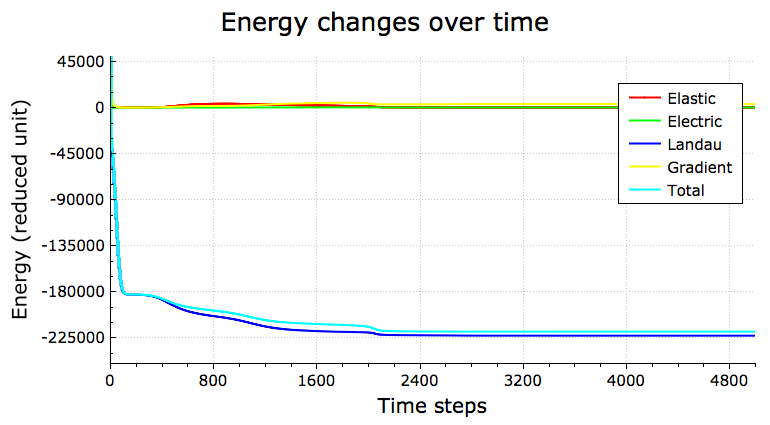
\includegraphics[width=0.8\textwidth]{img/energy-bulk.png}
\caption{How energy components vary with time}
\label{fig:example1-energy}
\end{center}
\end{figure}

If we use the second column as x axis and 3 to 8 columns as y axis to plot the changes of energy components in the whole system with respect to time steps, as it is shown in Figure \ref{fig:example1-energy}. We can see that after about 2500 steps, the total free energy flatten out and never decrease any more. You should be careful that energy reach a plateau does not necessarily mean you have found the most stable structure of lowest energy. It may be merely a metastable structure, that the driving force of polarization is not large enough to kick the domain configuration out of this local minima. In this example, though we start from random noise, the final domain structure is extremely simple, as shown in figure \ref{fig:example1-domain}. For this case, it is safe to say that what we have got is a stable domain structure. Otherwise, you should always try several different random seed to make sure what you have got is the most stable pattern. The two domains in figure \ref{fig:example1-domain} are two tetragonal domains, the yellow one is C+ domain and the black one is a2+ domain, each occupies 50\% of the whole system.

\begin{figure}[htbp]
\begin{center}
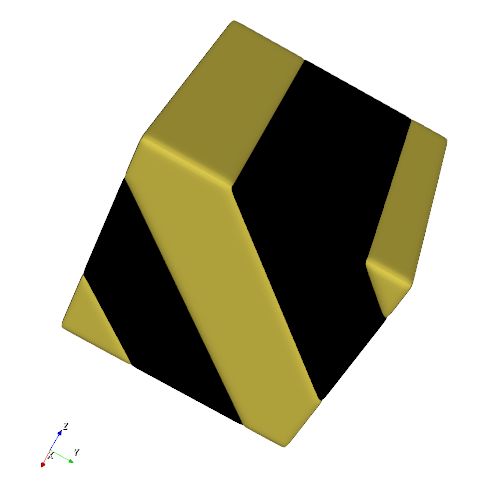
\includegraphics[width=0.33\textwidth]{img/domain-bulk.png}
\caption{The final stable domain structure}
\label{fig:example1-domain}
\end{center}
\end{figure}

After checking of the domain structure, you might want to take a look at the distribution of electric related variables such as electric potential, charges, electric field and electric energy, as well as elastic related variables such as total strain, eigenstrain, stress, elastic driving force and elastic energy.  All of these output files can be helpful under different using situations. The ones that we strongly recommend you to visualize in 3D and investigate whether the distribution is reasonable or meets your expectation, are charge, electric potential and stress distributions. The reasons are, first, checking their distribution can let you know if you are on the right track for simulation, and whether any parameters need to be further changed before you do a lot of trials and finally realize something seems not correct or you are not changing the most relevant parameter, second, compare these relatively straight forward variables to your expectation can be help you gain better feeling and understanding of the ferroelectric system, since electric and elastic contribution are extremely important to ferroelectric domain structures, they are the tool you have at hands to manipulate ferroelectric domains and in many cases helps to explain why some domain patterns are more favorable.

\begin{figure}[h]
\centering
\begin{subfigure}{0.33\textwidth}
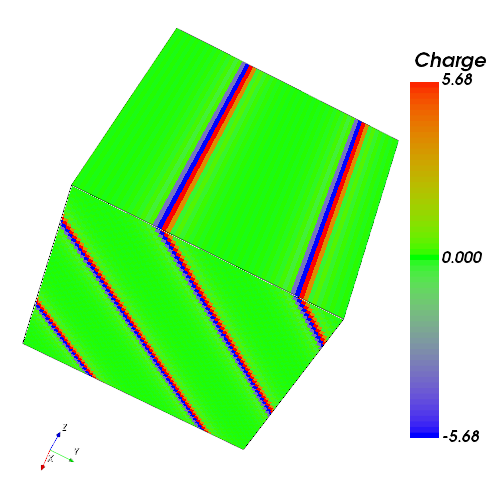
\includegraphics[width=\textwidth]{img/charge-bulk.png}
\caption{Bound charge }
\label{fig:example1-charge}
\end{subfigure}
\begin{subfigure}{0.33\textwidth}
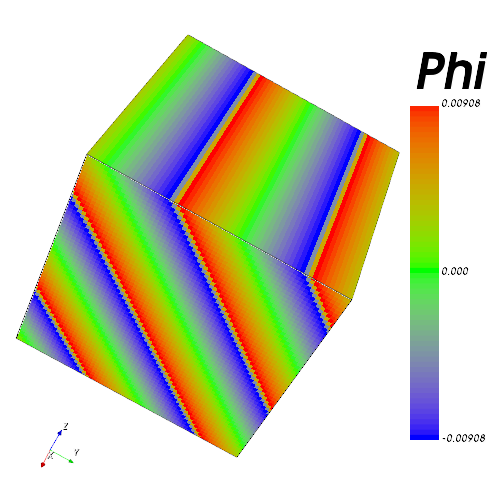
\includegraphics[width=\textwidth]{img/phi-bulk.png}
\caption{Electric potential }
\label{fig:example1-phi}
\end{subfigure}
\caption{Distribution of electric related variables}
\label{fig:example1-electric}
\end{figure}

The charge distribution and electric potential distribution is shown in figure \ref{fig:example1-electric}. From which we can see, the bound charges are mainly distributed along the domain wall. This meets our expectation, because inside a domain the polarization are the same, so there should be no bound charge. While for domain wall, as the polarization is varying, inevitably some bound charge will appear. The electric potential distribution might seems surprising at first glance, but when you read the legend, you will realize that the scale of this potential is very small.

\begin{figure}[h]
\centering
\begin{subfigure}{0.2\textwidth}
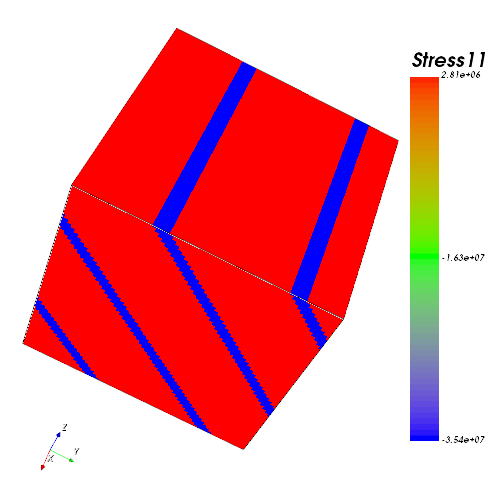
\includegraphics[width=\textwidth]{img/stress11-bulk.png}
\caption{$\sigma_{11}$ }
\label{fig:example1-stress11}
\end{subfigure}
\begin{subfigure}{0.2\textwidth}
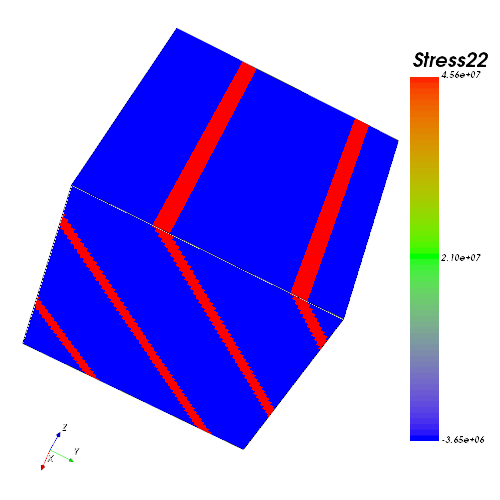
\includegraphics[width=\textwidth]{img/stress22-bulk.png}
\caption{$\sigma_{22}$}
\label{fig:example1-stress22}
\end{subfigure}
\begin{subfigure}{0.2\textwidth}
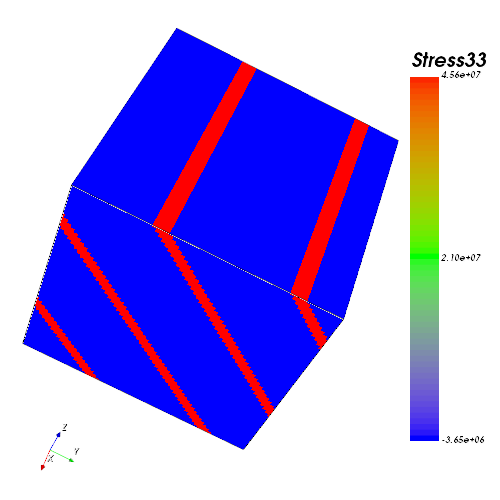
\includegraphics[width=\textwidth]{img/stress33-bulk.png}
\caption{$\sigma_{22}$}
\label{fig:example1-stress22}
\end{subfigure}

\begin{subfigure}{0.2\textwidth}
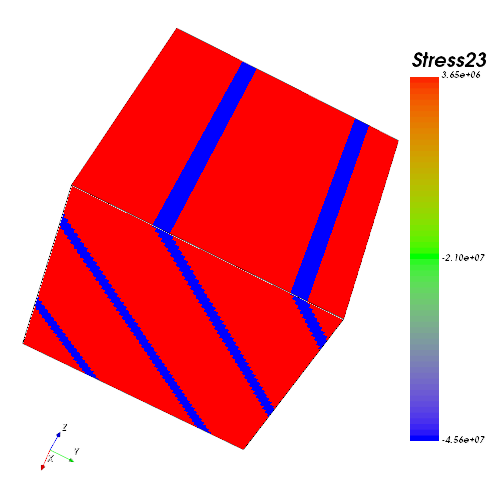
\includegraphics[width=\textwidth]{img/stress23-bulk.png}
\caption{$\sigma_{23}$ }
\label{fig:example1-stress23}
\end{subfigure}
\begin{subfigure}{0.2\textwidth}
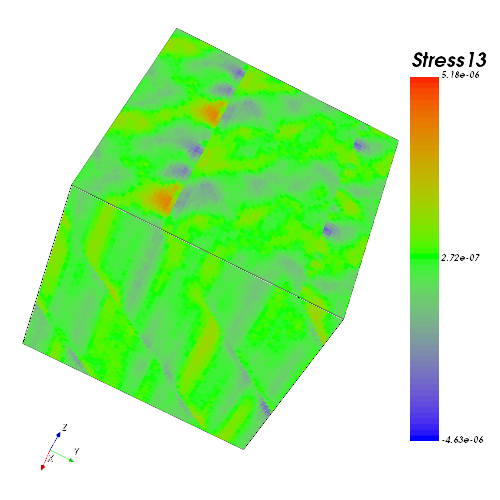
\includegraphics[width=\textwidth]{img/stress13-bulk.png}
\caption{$\sigma_{13}$}
\label{fig:example1-stress13}
\end{subfigure}
\begin{subfigure}{0.2\textwidth}
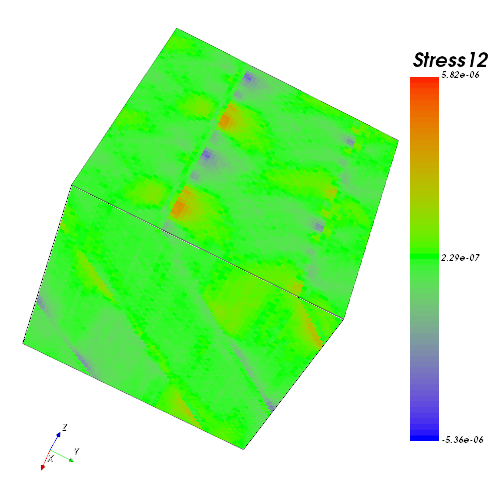
\includegraphics[width=\textwidth]{img/stress12-bulk.png}
\caption{$\sigma_{12}$}
\label{fig:example1-stress12}
\end{subfigure}
\caption{Stress distribution}
\label{fig:example1-stress}
\end{figure}

Due to the occurrence of a2+ and C+ domain, and the stress free boundary condition we applied, the distribution of $\sigma_{22}$, $\sigma_{33}$ and $\sigma_{23}$ is reasonable. $\sigma_{11}$ appears through the interaction with $\sigma_{22}$ and $\sigma_{33}$. The two x direction related shear stress, $\sigma_{13}$ and $\sigma_{12}$ , are 0 because all domains are tetragonal domains, shear strain can only be induced by the domain wall and as there is no a1 domains, no a1 related domain walls exist to introduce x direction related shear stress into the simulation system. You can consider this 3D simulation as an extension of 2D a2+ and C+ domains, and then the reason for missing $\sigma_{13}$ and $\sigma_{12}$ should become clear. 

For most of you simulations, the domain structure will be more complicated than it is in this example. You may not be able to perform such straight forward analysis of stress distribution. In that case, it is a good idea to study the elastic dirving force first, which is more directly related to polarization. 

Another thing you should remember is, in this ferroelectric module, we are only solving an elastic mechanical equilibrium equation, $\sigma_{ij,j}=0$, no plasticity, no large deformation is involved. In this scenario, stress is calculated from elastic strain, which is the difference between total strain and eigen strain, $\sigma_{kl} = C_{ijkl}(\epsilon_{ij}-\epsilon_{ij}^0)$, you can read this solid reference from Dr. Li published in 2002 for more details \cite{li2002elastic}.


% \section{Domain structure of BaTiO\textsubscript{3} thin film under different substrate mismatch strain}

\chapter{Recommended references}
\label{recom-refs}
\section{Potential related}
\begin{enumerate}
    

\item \textbf{Appendix A of the book "Physics of ferroelectrics: a modern perspective".}\cite{rabe2007physics}
\begin{quotation}
\em
In this appdendix, the landau potential and several important physical properties that are essential to phase-field simulation are provided for many materials.
\end{quotation}

\item \textbf{A phenomenological thermodynamic potential for BaTiO\textsubscript{3} single crystals.}\cite{li2005phenomenological}
\begin{quotation}
\em
An eighth order polynomial of Landau-Devonshire expansion was employed, which reproduce bulk properties including the three possible ferroelectric transition temperature and their dependence on electric fields, as well as the dielectric and piezoelectric constants. This potential is also applicable to thin films under large compressive biaxial strains.
\end{quotation}

\item \textbf{Temperature-pressure phase diagram and ferroeletric properties of BaTiO\textsubscript{3} single crystal based on a modified landau potential.}\cite{wang2010temperature}
\begin{quotation}
\em
A modified eight order landau potential was proposed for the BaTiO\textsubscript{3} by taking into account the quantum mechanical effects at low temperature, and the influence of hydrostatic pressure.
\end{quotation}

\item \textbf{A modified landau-devonshire thermodynamic potential for strontium titanate.}\cite{sheng2010modified}
\begin{quotation}
\em
Experiment results of strained thin film and phase-field simulations are used to refine the values of landau energy coefficient.
\end{quotation}

\item \textbf{Tuning the remanent polarization of epitaxial ferroelectric thin films with strain.}\cite{zhang2009tuning}
\begin{quotation}
\em
The effect of biaxial strain on the remanent polarization of epitaxial thin films of various ferroelectric materials is studied using phenomenological Landau-Devonshire theory.
\end{quotation}



\item \textbf{Computer simulation of ferroelectric domain stuctures in epitaxial BiFeO\textsubscript{3} thin films.}\cite{zhang2008computer}
\begin{quotation}
\em
Domain structure of (001), (101) and (111) oriented expitaxial BiFeO\textsubscript{3} thin films were studied. 
\end{quotation}
\end{enumerate}

\section{Elastic related}
\begin{enumerate}
    \item \textbf{Effect of substrate constraint on the stability and evolution of ferroelectric domain structures in thin films.}\cite{li2002elastic}. 
\begin{quotation}
The stability and evolution of ferroelectric domain structures in thin films are studied. Elastic solution are derived for both elastically anisotropic and isotropic thin films with arbitrary domain structures, subject to the mixed stress free and constraint boundary conditions.
\end{quotation}
\end{enumerate}



\section{Electric related}
\begin{enumerate}
    \item \textbf{Effect of electrical boundary condition on ferroelectric domain structures in thin films.}\cite{li2002electric}
    \begin{quotation}
    The effect of electrical boundary conditions on the domain morphologies and volume fractions are studied. It is shown that different electric boundary conditions may have a significant effect on the domain structures.
    \end{quotation}
    \item \textbf{Ferroelectric domain structures in SrBi\textsubscript{2}Nb\textsubscript{2}O\textsubscript{9} epitaxial thin films: Electron microscopy and phase-field simulations.}\cite{li2004ferroelectric}
    \begin{quotation}
    The effects of ferroelastic distortion and dielectric constant on ferroelectric domains are systematically analyzed. It is demonstrated that electrostatic interactions which favor straight domain walls are not sufficient to overcome the domain wall energy which favors curved domains in SrBi\textsubscript{2}Nb\textsubscript{2}O\textsubscript{9}.
    \end{quotation}
    \item \textbf{Phase-field simulation of polarization switching and domain evolution in ferroelectric polylcrystals.}\cite{choudhury2005phase}
    \begin{quotation}
    A phase-field model is developed for predicting the polarization switching and domain structure evolution under an applied electric field in ferroelectric polycrystals. A hysteresis loop, average polarization as a function of applied electric field, is computed, and the detailed domain evolution process during switching is analyzed.
    \end{quotation}
\end{enumerate}




\section{Tip related}
\begin{enumerate}
\item \textbf{Effect of ferroelastic twin walls on local polarization switching: Phase-field modeling.}\cite{choudhury2008effect}
\begin{quotation}
Local polarization switching in epitaxial ferroelectric thin films in the presence of ferroelastic domain walls was studied using phase-field approach. The nucleation bias profile across a twin wall was analyzed, and the localization of preferential nucleation sites was established.
\end{quotation}
\item \textbf{Nanoscale mechanical switching of ferroelectric polarization via flexoelectricity.}\cite{gu2015nanoscale}
\begin{quotation}
We examine the competition between pizeoelectric and flexoelectric effects and provide an understanding of the role of flexoelectricity in the polarization switching.
\end{quotation}
\end{enumerate}






\medskip

\bibliographystyle{unsrt}
\bibliography{mupro-ferro}

\end{document}




